\chapter{Kerr black holes with Proca hair}
\label{ch:proca}

\epigraph{``\emph{
Ein sat hún úti \\
þá er inn aldni kom \\
yggjungur ása \\
og í augu leit: \\
„Hvers fregnið mig? \\
Hví freistið mín?“ \\
Allt veit eg, Óðinn, \\
hvar þú auga falt, \\
í inum mæra \\
Mímisbrunni. \\
Drekkur mjöð Mímir \\
morgun hverjan \\
af veði Valföðurs. \\
Vituð ér enn eða hvað? 
} 
''}{28th verse of Völuspá}


%%%%%%%%%%%%%%%%%%%%%%%%%%%%%%%%%%%%%%%%%%%%%%%%%%%%%%%%%%%%%%%%%%%%%%%%%%%%%%%
\section{Introduction}
% %%%%%%%%%%%%%%%%%%%%%%%%%%%%%%%%%%%%%%%%%%%%%%%%%%%%%%%%%%%%%%%%%%%%%%%%%%%%%%%
%  
% In vacuum General Relativity (GR) black holes (BH) are remarkably simple. The Carter-Robinson theorem~\cite{Carter:1971zc,Robinson:1975bv}, supplemented by the rigidity theorem~\cite{Hawking:1971vc,Racz:1995nh}, established that asymptotically flat, stationary, non-singular (on and outside an event horizon)  \textit{vacuum} BHs of GR have \textit{only} 
% two degrees of freedom -- see~\cite{Chrusciel:2012jk} for a review.  
%
% The most general BH solution in this context is the Kerr metric~\cite{Kerr:1963ud} and the two degrees of freedom are the ADM mass, $M$, and angular momentum, $J$, both of which can be determined by an observer at infinity. 
%
% The natural question of how this result generalizes in the presence of matter led to the \textit{no-hair} hypothesis~\cite{Ruffini:1971bza}: regardless of the matter involved, the end-point of gravitational collapse -- in GR and in an astrophysical context -- is characterized solely by conserved charges associated to Gauss laws, including $M,J$, and no further parameters (\textit{hair}). Thus, an observer at infinity should be able to fully compute all relevant ``charges" of an equilibrium BH.
%
% Evidence in favour of this hypothesis has been presented in terms of \textit{no-hair theorems} for particular matter models in GR. A collection of such theorems for the much studied case of scalar matter can be found in the recent review~\cite{Herdeiro:2015waa}. Of relevance for the present paper, Bekenstein established a no-Proca hair theorem for stationary BH solutions of Einstein's gravity minimally coupled to one (or more) real, Abelian Proca field~\cite{Bekenstein:1971hc,Bekenstein:1972ky}, which will be reviewed in Section~\ref{sec_nohair1}. 
%
%
%
% Evidence against the no-hair hypothesis in asymptotically flat spacetimes, on the other hand, has been presented in the form of hairy BH solutions, starting with the pioneering examples in Yang-Mills theory~\cite{Volkov:1998cc} (see also the reviews~\cite{Bizon:1994dh,Bekenstein:1996pn,Herdeiro:2015waa,Volkov:2016ehx}). 
% Such counter-examples, however, typically either 
% 1) violate some energy condition ($e.g.$~\cite{Nucamendi:1995ex,Bechmann:1995sa,Anabalon:2013qua,Anabalon:2012ih,Cadoni:2015gfa}); or 
% 2) have non-minimal couplings between matter and geometry ($e.g.$~\cite{Bekenstein:1975ts,Bekenstein:1974sf,BBM,Sotiriou:2014pfa,Sotiriou:2013qea,Babichev:2013cya}); or 
% 3) have non-canonical/non-linear kinetic terms ($e.g.$~\cite{Luckock:1986tr,Luckock,Bronnikov:2005gm,Radu:2011uj}); or 
% 4) the hair is not independent of other fields, such as an electromagnetic field (secondary hair, $e.g.$~\cite{Gibbons:1987ps,Gibbons:1982ih}); or 
% 5) involve higher curvature terms 
% ($e.g$~\cite{Kanti:1995vq,Ayzenberg:2014aka,Kleihaus:2011tg,Kleihaus:2015aje,Pani:2011gy,Pani:2009wy,Alexander:2009tp,Yunes:2009hc}); or 
% 6) several of the above. It is unclear, moreover, if any of these counter-examples violates the \textit{dynamical spirit} of the no-hair hypothesis; that is, if there are dynamically stable hairy BHs that can be the end-point (or be sufficiently long lived) in a dynamical evolution.
%
% \bigskip
%
% In a qualitatively novel development, a class of BH solutions with scalar hair was found in 2014 bifurcating from the Kerr metric~\cite{Herdeiro:2014goa}: \textit{Kerr BHs with scalar hair} (KBHsSH).
% %
%  These are solutions of the simple model
%  \begin{equation}
% \label{actionscalar}
% S=\int  d^4x \sqrt{-g}\left[ \frac{R}{16\pi G}
%    -\frac{g^{\alpha\beta}}{2} \left( \Psi_{, \, \alpha}^* \Psi_{, \, \beta} + \Psi _
% {, \, \beta}^* \Psi _{, \, \alpha} \right) - \mu^2 \Psi^*\Psi
% %( \left| \Phi \right|) 
%  \right]  \ ,
% \end{equation}
% that 1) obey all energy conditions; 2) have minimal couplings with the geometry; 3) have canonical kinetic terms; 4) have an independent (primary) hair; 5) exist in GR, without higher curvature terms. KBHsSH, moreover, are asymptotically flat, regular on and outside the event horizon, reduce to (specific) Kerr solutions in the limit of vanishing hair, and to gravitating solitons known as \textit{boson stars}~\cite{Schunck:2003kk,Liebling:2012fv} in the limit of vanishing horizon. The scalar hair is described by an independent  conserved Noether charge \textit{but without} an associated Gauss law. Thus, an observer at infinity cannot determine this charge -- which must be computed by a volume integral -- and hence does not have access to all the relevant spacetime charges.  
%
The matter content for the original example in~\cite{Herdeiro:2014goa} (see also~\cite{Herdeiro:2015gia}) was a massive complex scalar field, $cf.$~\eqref{eqn:HBH-ansatz}.
The connection between KBHsSH and superradiance led to the suggestion that, underlying the example of KBHsSH, there is a more general mechanism~\cite{Herdeiro:2014goa,Herdeiro:2014ima} (see also~\cite{Herdeiro:2015waa,Herdeiro:2015gia}): 
{\bf Conjecture:}
\begin{description}
\item[1)] If a ``hairless" stationary BH spacetime $(\mathcal{M}_0,{\bf g_0})$ is afflicted by superradiant instabilities triggered by a given test field $\mathcal{F}$;
\item[2)] If the field modes at the threshold of the instability (zero modes), $\mathcal{F}_t$, yield an energy-momentum tensor $\mathcal{T}(\mathcal{F}_t,\mathcal{F}_t)$ which is time-independent $\mathcal{L}_{\bf k}\mathcal{T}(\mathcal{F}_t,\mathcal{F}_t)=0$, where ${\bf k}$ is the time-like Killing vector field (at infinity) that preserves the metric $\mathcal{L}_{\bf k}{\bf g_0}=0$;
\item[Then:] there is a new family of stationary BH ``hairy solutions" bifurcating from $(\mathcal{M}_0,{\bf g_0})$, denoted by $(\mathcal{M}_\mathcal{F},{\bf g_\mathcal{F}})$. Actually, $(\mathcal{M}_\mathcal{F},{\bf g_\mathcal{F}})$ may be a countable set of families.
\end{description}
In the case of KBHsSH, one encounters a family with three continuous and two discrete degrees of freedom.

As further evidence for the above conjecture we consider now 
Einstein's gravity minimally coupled to Abelian Proca fields, hereafter referred simply as Proca fields\footnote{Gravitating \textit{non-Abelian} ($SU(2)$) Proca fields have been studied in \cite{Greene:1992fw}, wherein spherically symmetric solitons and BHs have been discussed. The properties of these solutions are rather distinct from the solutions discussed in this chapter and, moreover, the former have not been generalized to include rotation.}. 
Massive Proca fields trigger, in much the same way as massive scalar fields, 
superradiant instabilities of Kerr BHs -- see~\cite{Pani:2012vp,Pani:2012bp,Witek:2012tr} 
for recent studies of Proca-induced superradiant instabilities in asymptotically flat BHs. 

%% Adjust the paragraph below to fit into the paper or skip it? Not sure if writing a summary of each chapter in the introduction is needed.

% This paper is organized as follows. In Section~\ref{Psec_model} we exhibit the Einstein--complex-Proca model and its basic properties. In Section~\ref{sec_nohair} we review the classic no-Proca-hair theorem by Bekenstein~\cite{Bekenstein:1971hc,Bekenstein:1972ky} and also present a novel no-Proca-hair theorem applying to \textit{spherically symmetric} solutions and allowing the Proca field to have a harmonic time dependence. The latter is a generalization of the theorem presented in~\cite{Pena:1997cy} for the scalar case and it establishes that rotation is crucial for the existence of KBHsPH. In Section~\ref{sec_clouds} we consider the construction of stationary Proca clouds around Kerr and obtain one existence line for a particular set of ``quantum" numbers. In Section~\ref{sec_stars} we shall briefly review some of the main features of Proca stars, that form a limiting case of KBHsPH, and discuss some of their physical properties in the rotating case. In Section~\ref{sec_kbhsph} we finally construct KBHsPH, discussing the ansatz, boundary conditions and solving numerically the field equations. Then we exhibit the domain of existence and phase space of one family of solutions, we discuss the Proca energy spacetime distribution and some other physical features of these BHs. We close with a discussion of the results of this paper and some of the open directions for future related research.  In the Appendices we provide some technical results, including the explicit expression for the Einstein tensor, Proca energy-momentum tensor and Proca field equations.
%
%

 %%%%%%%%%%%%%%%%%%%%%%%%%%%%%%%%%%%%%%%%%%%%%%%%%%%%%%%%%%%%%%%%%%%%%%%%%%%%%%%
\section{Einstein--complex-Proca model}
\label{Psec_model}
%%%%%%%%%%%%%%%%%%%%%%%%%%%%%%%%%%%%%%%%%%%%%%%%%%%%%%%%%%%%%%%%%%%%%%%%%%%%%%% 
The field equations for a massive vector field were introduced by A. Proca~\cite{Proca} in the 1930s. Much more recently, gravitating Proca fields have been discussed by various authors -- see $e.g.$~\cite{Rosen:1994rq,Obukhov:1999ed,Toussaint:1999zz}. Here, we shall consider  two real Proca fields, both with mass $\mu$, but our discussion can be easily generalized to an arbitrary even number of real Proca fields (or an arbitrary number of complex ones). 
The two fields are described by the potential 1-forms $A^{(i)}$, $i=1,2$, and field strengths $F^{(i)}=dA^{(i)}$. It is convenient to organize them into a single complex Proca field:
\begin{equation}
\mathcal{A}=A^{(1)}+iA^{(2)} \ , \qquad \mathcal{F}=F^{(1)}+iF^{(2)} \ .
\end{equation}
We denote the complex conjugate by an overbar,
\begin{equation}
\bar{\mathcal{A}}=A^{(1)}-iA^{(2)} \ , \qquad \bar{\mathcal{F}}=F^{(1)}-iF^{(2)} \ .
\end{equation}
Considering that the two Proca fields do not couple to each other and couple minimally to gravity, one obtains the minimal Einstein--complex-Proca model, which is  
described by the action:
\begin{equation}
\label{Procaaction}
\mathcal{S}=\int d^4x \sqrt{-g}\left(\frac{1}{16 \pi  G}R
-\frac{1}{4}\mathcal{F}_{\alpha\beta}\bar{\mathcal{F}}^{\alpha\beta}
-\frac{1}{2}\mu^2\mathcal{A}_\alpha\bar{\mathcal{A}}^\alpha\right) \ .
\end{equation}
This (or its version with $A_\alpha$ real) 
is the action considered by previous studies of the Einstein-Proca model, see
$e.g.$ refs. \cite{Rosen:1994rq,Vuille:2002qz}.\footnote{We remark that these works did not succeed in finding regular particle-like solutions or BHs with Proca hair.}

Varying  (\ref{Procaaction}) $w.r.t.$ the potential $A_\alpha$ yields the Proca field equations
\begin{equation}
\nabla_\alpha\mathcal{F}^{\alpha\beta}=\mu^2 \mathcal{A}^\beta \ .
\label{procafe}
\end{equation}
Observe that these equations \textit{completely} determine $ \mathcal{A}^\beta$ once $\mathcal{F}^{\alpha\beta}$ is known. Thus, the Proca potential is not subject to gauge transformations, unlike the Maxwell potential, and it is as physical as the field strength. In particular \eqref{procafe} imply the Lorentz condition, thus a dynamical requirement, rather than a gauge choice:
\begin{equation}
\nabla_\alpha\mathcal{A}^\alpha = 0 \ .
\label{lorentz}
\end{equation}


As usual, the Einstein equations are found by taking the variation of
(\ref{Procaaction}) $w.r.t.$ the metric tensor $g_{\alpha \beta}$
\begin{equation}
R_{\alpha \beta}-\frac{1}{2}R g_{\alpha \beta}=8 \pi G T_{\alpha \beta} \ ,
\label{Einstein-eqs}
\end{equation}
where the energy-momentum tensor reads:
\begin{eqnarray}
T_{\alpha\beta}=\frac{1}{2}
( \mathcal{F}_{\alpha \sigma }\bar{\mathcal{F}}_{\beta \gamma}
+\bar{\mathcal{F}}_{\alpha \sigma } \mathcal{F}_{\beta \gamma}
)g^{\sigma \gamma}
-\frac{1}{4}g_{\alpha\beta}\mathcal{F}_{\sigma\tau}\bar{\mathcal{F}}^{\sigma\tau}+\frac{1}{2}\mu^2\left[  
\mathcal{A}_{\alpha}\bar{\mathcal{A}}_{\beta}
+\bar{\mathcal{A}}_{\alpha}\mathcal{A}_{\beta}
-g_{\alpha\beta} \mathcal{A}_\sigma\bar{\mathcal{A}}^\sigma\right]\ . \ \ \ \ \ \ \  \ 
\label{procaemt}
\end{eqnarray}

The action possesses a global $U(1)$ symmetry, since it is invariant under the transformation 
$\mathcal{A}_\beta\rightarrow e^{i\chi}\mathcal{A}_\beta$, with $\chi$ constant; 
this implies the existence of a  4-current, 
%
\begin{equation}
\label{j}
j^\alpha=\frac{i}{2}\left[\bar{\mathcal{F}}^{\alpha \beta}\mathcal{A}_\beta-\mathcal{F}^{\alpha\beta}\bar{\mathcal{A}}_\beta\right] \ ,
\end{equation}
which is conserved by virtue of the field equations (\ref{procafe}): $\nabla_\alpha j^\alpha=0$. Consequently, there exists a Noether charge, $Q$, obtained integrating the temporal component of the 4-current on a space-like slice $\Sigma$:
\begin{equation}
Q=\int_\Sigma d^3x j^0 \ .
\label{Pq}
\end{equation}
We emphasize that unlike the massless limit of the theory, wherein the global symmetry becomes local, the last integral cannot be converted into a surface integral. In other words, there is no Gauss law.


 
 %%%%%%%%%%%%%%%%%%%%%%%%%%%%%%%%%%%%%%%%%%%%%%%%%%%%%%%%%%%%%%%%%%%%%%%%%%%%%%%
\section{No Proca-hair theorems}
\label{sec_nohair}
%%%%%%%%%%%%%%%%%%%%%%%%%%%%%%%%%%%%%%%%%%%%%%%%%%%%%%%%%%%%%%%%%%%%%%%%%%%%
If one considers Maxwell's equations for a test field with a spherically symmetric ansatz (a purely radial electric field) on the Schwarzschild background one finds a regular solution on and outside the Schwarzschild horizon ($cf.$ Section 2.1 in~\cite{Herdeiro:2015waa}). This is a smoking gun that a spherically symmetric field can be added, non-linearly, to the Schwarzschild solution, which indeed yields the well-known Reissner-Nordstr\"om BH. 
Adding a mass term to the Maxwell field -- hence converting it into a Proca field -- drastically alters the behaviour of the test field solution: it is not possible to find a solution which is both finite at the horizon and at spatial infinity, no matter how small $\mu$ is. 
In particular, for the asymptotically (exponentially) decaying solution, the Proca potential squared diverges at the horizon~\cite{Gottlieb:1984jg}.
Thus, requiring any amount of Proca field in equilibrium outside the horizon implies an infinite pile up of Proca invariants at the horizon.
This behaviour parallels that of a scalar field (massless or massive) discussed in~\cite{Herdeiro:2015waa} and it is intimately connected with the existence/absence of a Gauss law for the Maxwell/Proca field.
Moreover, it shows one cannot find a regular, spherically symmetric BH solution with Proca (time-independent) hair bifurcating from the Schwarzschild solution.

Just as with KBHsSH, a key assumption in finding Kerr black holes with Proca hair is to violate the assumption of many no-hair theorems that the field inherits the isometries of the background.
In \cite{Herdeiro:2016tmi}, it was shown that even dropping the symmetry inheritance assumption one can establish a no-hair theorem, for \textit{spherically symmetric} BHs.
This is compatible with the KBHsPH solutions discussed in this chapter, which are stationary and axi-symmetric, and shows that these solutions cannot have a static limit,
as can be seen from the domain of existence of KBHsPH, $cf.$ Section~\ref{subsec_III}.

%
% %%%%%%%%%%%%%%%%%%%%%%%%%%%%%%%%%%%
% \subsection{Bekenstein's theorem}
% \label{sec_nohair1}
% %%%%%%%%%%%%%%%%%%%%%%%%%%%%%%%%%%%%%%%%%%%%%%%%%%%%%%%%%%%%%%%%%%%%%%%%%%%%
% Following Bekenstein~\cite{Bekenstein:1971hc,Bekenstein:1972ky}, we consider a rotating, stationary, asymptotically flat BH spacetime. For matter obeying the null energy condition, the rigidity theorem implies that the spacetime is also axi-symmetric~\cite{Hawking:1971vc}. We write the spacetime metric in coordinates adapted to these symmetries $(t,r,\theta,\phi)$, so that the two Killing vector fields read ${\bf k}=\partial_t$, ${\bf m}=\partial_\phi$.
%
%
% For simplicity we consider the Proca field to be real. But the proof generalizes straightforwardly for an arbitrary number of real Proca fields, and in particular for a complex Proca field. We denote the real Proca potential and field strength as $A_\alpha$ and $F_{\alpha\beta}$, respectively. We assume that this field inherits the spacetime symmetries. In particular for the coordinates chosen above 
% this means that: 
% \begin{equation}
% \mathcal{L}_{\bf k} A_\alpha=\mathcal{L}_{\bf m} A_\alpha=0=\mathcal{L}_{\bf k} F_{\alpha\beta}=\mathcal{L}_{\bf m} F_{\alpha\beta} \ .
% \label{symmetriesaf}
% \end{equation}
%
% The proof proceeds as follows. We contract the Proca equation $\nabla_\alpha F^{\alpha\beta}=\mu^2 A^\beta$ with $A_\beta$ and integrate over the BH exterior space-time:
% \begin{equation}
% \int d^4x\sqrt{-g}\left[A_\beta\nabla_\alpha F^{\alpha\beta}-\mu^2 A_\beta A^\beta\right]=0 \ .
% \end{equation}
% Next, integrating the first term by parts:
% \begin{equation}
% \int d^4x\sqrt{-g}\left[\frac{F_{\alpha\beta} F^{\alpha\beta}}{2}+\mu^2 A_\beta A^\beta\right]-\int_{\mathcal{H}}d^3\sigma n^\alpha A_\beta F_{\alpha}^{\ \beta}=0 \ ,
% \label{bek1}
% \end{equation}
% where the boundary term is computed on the (spatial section of the) horizon, $\mathcal{H}$, and the other boundary term (at infinity) vanishes since the Proca field falls off exponentially fast.
%
% Now we argue that the boundary term in  \eqref{bek1} is zero. To do so, we first observe that defining $b_\alpha\equiv A_\beta F_{\alpha}^{\ \beta}$, then $b_t=0=b_\phi$. This results from the symmetries imposed, which imply $A_r=A_\theta=F_{r\theta}=F_{t\phi}=0$.\footnote{$F_{t\phi}=0$ follows immediately from~\eqref{symmetriesaf}. Non-vanishing $A_r,A_\theta,F_{r\theta}$ would imply non vanishing components $T_{tr}$ and $T_{t\theta}$ of the energy momentum tensor~\eqref{procaemt}, which are incompatible with the symmetries of the problem.} 
% Since, the event horizon of a stationary, asymptotically flat spacetime is a Killing horizon, the normal to $\mathcal{H}$, $n^\alpha$, 
% is a linear combination of the Killing vector fields. Then $n^\alpha A_\beta F_{\alpha}^{\ \beta}=0$. 
% %
% We conclude that\footnote{We are implicitly assuming that $d^3\sigma$ and $A_\alpha,F_{\alpha\beta}$ are finite on $\mathcal{H}$. This assumption actually breaks down for the massless case (Maxwell field) due to gauge invariance.}
% \begin{equation}
% \int d^4x\sqrt{-g}\left[\frac{F_{\alpha\beta} F^{\alpha\beta}}{2}+\mu^2 A_\beta A^\beta\right]=0 \ .
% \label{bek3}
% \end{equation}
%
% Contrary to the scalar field case (see $e.g.$~\cite{Herdeiro:2015waa}) this integrand is not positive definite. Thus, a further argument is necessary, which can be constructed by using an orthonormal basis, which we denote as $\{ {\bf e}^{\underline{t}},{\bf e}^{\underline{r}},{\bf e}^{\underline{\theta}},{\bf e}^{\underline{\phi}}\}$. Flat (underlined) indices are raised and lowered with the standard Cartesian Minkowski metric. Taking into account the allowed components by symmetry of the Proca potential and field strength, \eqref{bek3} becomes:
% \begin{equation}
% \begin{array}{l}
% \displaystyle{\int d^4x\sqrt{-g}\left[(F_{\underline{t}\underline{r}})^2+(F_{\underline{t}\underline{\theta}})^2+(A_{\underline{t}})^2\right]} \displaystyle{=\int d^4x\sqrt{-g}\left[(F_{\underline{\phi}\underline{r}})^2+(F_{\underline{\phi}\underline{\theta}})^2+(A_{\underline{\phi}})^2\right]} \ .
% \end{array}
% \label{procaproof}
% \end{equation}
% Analysing the time-reversal invariance of the Proca equation, shows that $\{F_{\underline{t}\underline{r}},F_{\underline{t}\underline{\theta}},A_{\underline{t}}\}$ are even, whereas $\{F_{\underline{\phi}\underline{r}},F_{\underline{\phi}\underline{\theta}},A_{\underline{\phi}}\}$ are odd, under time-reversal. Thus, expanding the Proca potential and field strength in a power series of the angular momentum of the background, the first (second) set of field/potential components contains only even (odd) powers. The zeroth order terms only get contributions from the left hand side of \eqref{procaproof}; since the corresponding integrand is strictly positive and the integral is zero, the zeroth order terms must vanish. Then, the first order terms only get contributions from the right hand side of \eqref{procaproof}; since the corresponding integrand is strictly positive and the integral is zero, the first order terms must vanish. In this way one shows iteratively that the Proca field/potential must vanish, and hence there is no Proca hair. 
% Observe that this theorem did not use the Einstein equations.
%
% A different proof of the no Proca-hair theorem, possibly including a cosmological constant  and making use of the Einstein equations, 
% has been given in \cite{Bhattacharya:2011dq}.
%
%
%
%
%  %%%%%%%%%%%%%%%%%%%%%%%%%%%%%%%%%%%%%%%%%%%%%%%%%%%%%%%%%%%%%%%%%%%%%%%%%%%%%%%
% \subsection{A modified Pe\~{n}a--Sudarsky theorem}
% \label{sec_nohair2}
% %%%%%%%%%%%%%%%%%%%%%%%%%%%%%%%%%%%%%%%%%%%%%%%%%%%%%%%%%%%%%%%%%%%%%%%%%%%%
% The theorem of the previous subsection relied on the symmetry inheritance of the spacetime isometries by the Proca field. In particular the stationarity of the geometry implied a time-independence of the Proca potential/field. Recently, however, gravitating solitons composed by self-gravitating Proca fields were found by allowing the complex Proca field to have a \textit{harmonic time dependence}: Proca stars~\cite{Brito:2015pxa}. This time-dependence vanishes at the level of the energy momentum tensor and it is therefore compatible with a stationary geometry (see~\cite{Smolic:2015txa} for recent discussions of symmetry inheritance). Thus one may wonder if allowing the Proca field to have such harmonic time dependence allows for BHs with Proca hair. 
%
% The situation just described parallels closely the well-known picture for complex scalar fields. The existence of scalar boson stars led Pe\~{n}a and Sudarsky to consider the possibility of spherically symmetric BH geometries with a scalar field possessing a harmonic time dependence. In this setup it was possible to establish a no-scalar-hair theorem, ruling out BHs with scalar hair even if the hair has such harmonic time-dependence~\cite{Pena:1997cy}. In the following we shall establish a no-Proca-hair theorem, allowing the complex Proca field to have a harmonic time dependence, for the case of spherical symmetry, by using a modified version of the arguments in~\cite{Pena:1997cy}. 
%
% We consider a spherically symmetric line element with the parametrization (see $e.g.$~\cite{Brito:2015pxa}):
% %
% \begin{equation}
% ds^2=-\sigma^2(r)N(r)dt^2+\frac{dr^2}{N(r)}+r^2d\Omega_2 \ ,  \qquad \ N(r)\equiv 1-\frac{2m(r)}{r} \ .
% \label{ansatz1}
% \end{equation}
% %
% The Ansatz we consider for the complex Proca potential is also the one introduced in \cite{Brito:2015pxa} for discussing spherical Proca stars and it is the most general one compatible with spherical symmetry and staticity:
% %
% \begin{equation}
% \mathcal{A}=e^{-iwt}\left[f(r)dt+ig(r)dr \right] \ .
% \label{ansatz2}
% \end{equation}
% %
% In the above relations, $\sigma(r),m(r),f(r),g(r)$ 
% are all real functions of the radial coordinate only and $w$ is the frequency parameter, which we take to
% be positive without any loss of generality. 
%
%  %
%  The Proca field equations~\eqref{procafe} yield 
%  \begin{equation}
%  \frac{d}{dr}\left\{\frac{r^2[f'(r)-wg(r)]}{\sigma(r)}\right\}=\frac{\mu^2r^2f(r)}{\sigma(r)N(r)} \ ,
%  \label{proca1}
%  \end{equation}
%  %
%  and
%  \begin{equation}
%  %wg(r)-f'(r)=\frac{\mu^2\sigma^2(r)N(r)g(r)}{w} \ .
%  f'(r)=wg(r) \left (1-\frac{\mu^2\sigma^2(r)N(r) }{w^2} \right) \ ,
%  \label{eq1}
%  \end{equation}
%  where ``prime" denotes radial derivative. The Lorentz condition, \eqref{lorentz}, determines $f(r)$ in terms of the other functions:
%  %
% \begin{equation}
% f(r)=-\frac{\sigma(r)N(r)}{wr^2}\frac{d}{dr}\left[r^2\sigma(r)N(r)g(r)\right] \ ;
% \label{lor}
% \end{equation} 
% this can be rewritten as
% \begin{equation}
% \frac{d}{dr}\left[r^2\sigma(r)N(r)g(r)\right] =-\frac{wr^2 f(r)}{\sigma(r)N(r)}\ .
% \label{eq2}
% \end{equation} 
%  Observe that (\ref{proca1})-(\ref{eq1}) imply (\ref{eq2}), as they should. 
%  %
% %
%  %
% The essential Einstein equations, \eqref{Einstein-eqs}, read (there is a further Einstein equation which is a differential consequence of these)
% \begin{eqnarray}
% \label{Einstein-eqs1}
% &&
% m'=4\pi G r^2
% \left[
% \frac{(f'-wg)^2}{2\sigma^2}
% +\frac{1}{2}\mu^2 \left(g^2N+\frac{f^2}{N\sigma^2}\right)
% \right], \nonumber 
% \\
% &&\frac{\sigma'}{\sigma}=4\pi G r  \mu^2
% \left(g^2+\frac{f^2}{N^2\sigma^2} \right).
% \end{eqnarray} 
% %
% We also note that the $T_t^t$ component of the energy-momentum tensor -- the
% energy density -- reads
%  \begin{equation}
% \label{ro}
% -T^t_t=
%  \frac{(f'-wg)^2}{2\sigma^2}
% +\frac{1}{2}\mu^2 \left(g^2N+\frac{f^2}{N\sigma^2} \right)\ .
% \end{equation}
%  
%
% To establish the no-Proca-hair theorem, let us assume the existence of a regular BH solution of the above  equations. Then the geometry would possess a non-extremal horizon at, say, 
% $r=r_H>0$, which requires that 
%  \begin{equation}
% N(r_H)=0 \ ,
% \end{equation}
% since $r=r_H$ is a null surface. Since we are assuming that there are no more exterior horizons, then $r>r_H=$constant are timelike surfaces and $N'(r_H)>0$. Also, we can choose without loss of generality that $\sigma(r_H)>0$, since the equations of motion are invariant under $\sigma\rightarrow -\sigma$. It follows that $N(r)$ and $\sigma(r)$ are strictly positive functions for any $r>r_H$, as a consequence of the Einstein equations~\eqref{Einstein-eqs1} and the assumption that there are no further more exterior horizons.
%
% The regularity of the horizon implies that the energy density of the Proca field
% is finite there.
% From (\ref{ro}) one can see that this implies
%  \begin{equation}
% f(r_H)=0\ .
% \end{equation}
% Then the function $f(r)$ starts from zero at the horizon 
% and remains strictly positive (or negative) for some $r$-interval.
% Now, let us assume $f'(r)>0$ for 
% $r_H<r<r_1$. Thus $f(r)$, in this interval, is a strictly increasing (and positive) function 
% (the case $f'(r)<0$ can  be discussed in a similar way).
%
% Next, we consider the expression (which appears in~\eqref{eq1}) 
%  \begin{equation}
% P(r)\equiv 1-\frac{\mu^2\sigma^2(r)N(r) }{w^2}\ .
% \end{equation}
% One can see that $P(r_H)=1$; actually $P$  
% becomes negative for large $r$, since $N\to 1$, $\sigma\to 1$ as $r\to \infty$, while $\mu>w$, which is a bound state condition necessary for an exponential decay of the Proca field at infinity. But the important point is the existence of an $r-$interval
% $r_H<r<r_2$ where $P$ is a strictly positive function.
%
%
% Let $r_c$ be the minimum between $r_1$ and $r_2$.
% Then   
%   we observe that (\ref{eq2}) implies
% \begin{equation}
%  r^2\sigma(r)N(r)g(r)  =-w\int_{r_H}^r\ dx \frac{x^2}{\sigma(x)N(x)} f(x)<0 
% \label{eq21}
% \end{equation} 
% for  any $r$ in the interval $r_H<r<r_c$. Consequently, $g(r)<0$ in this interval, since $\sigma,N$ are positive everywhere outside the horizon.
%
% The last conclusion implies a contradiction: $g(r)<0$ is not compatible with $f'(r)>0$, in that interval. In fact, $f'(r)>0$ together with $P>0$ and $w>0$, from (\ref{eq1}), that $g(r)>0$. 
% %The above assumptions imply
% %$wg(r) \left (1-\frac{\mu^2\sigma^2(r)N(r) }{w^2} \right)<0$ (since $P>0$, $w>0$, $g<0$)  and therefore $f'(r)<0$.
% Thus we conclude that $f(r)=g(r)=0$ is the only solution compatible with a BH geometry ($q.e.d.$). 
%
%
% One final observation concerning static fields ($w=0$). In such cases, one has only an electric potential, $g(r)=0$.
% Then, the Proca equations  on a Schwarzschild
% background -- $i.e.$ taking the line element (\ref{ansatz1}) 
% with $\sigma(r)=1$, $N(r)=1-2M/r$, --
% can be solved in closed form by taking the ansatz~\cite{Gottlieb:1984jg}
% \begin{equation}
% f(r)=\frac{e^{-\mu r}}{r}S(r) \ ,
% \label{eqs1}
% \end{equation} 
% where $S(r)$ is a solution of the Kummer equation~\cite{Abramowitz} 
% \begin{equation}
% z\frac{d^2 S(z)}{dz^2}-z \frac{d S(z)}{dz}-M \mu S(z)=0\ ,~~{\rm with}~~z\equiv 2\mu(r-2M) \ .
% \label{eqs2}
% \end{equation} 
% This equation possesses a solution which is regular on and outside the  horizon.
% In particular, $S(z)$ takes a constant nonzero value at $z=0$ ($i.e.$ $r=2M$).
% This implies, however, that the invariant $A_\mu A^\mu=-f^2(r)/(1-2M/r)$
% diverges at the horizon.
%
%
%
%  %%%%%%%%%%%%%%%%%%%%%%%%%%%%%%%%%%%%%%%%%%%%%%%%%%%%%%%%%%%%%%%%%%%%%%%%%%%%%%%
% %\subsection{Other no Proca-hair theorem arguments}
% %\label{sec_nohair3}
% %%%%%%%%%%%%%%%%%%%%%%%%%%%%%%%%%%%%%%%%%%%%%%%%%%%%%%%%%%%%%%%%%%%%%%%%%%%%
%
%
%  
%

 %%%%%%%%%%%%%%%%%%%%%%%%%%%%%%%%%%%%%%%%%%%%%%%%%%%%%%%%%%%%%%%%%%%%%%%%%%%%%%%
\section{Stationary Proca clouds around Kerr}
\label{sec_clouds}
%%%%%%%%%%%%%%%%%%%%%%%%%%%%%%%%%%%%%%%%%%%%%%%%%%%%%%%%%%%%%%%%%%%%%%%%%%%%%%% 
The theorems discussed in section~\ref{sec_nohair} leave open the possibility that \textit{stationary} (rather than static and spherically symmetric) BHs with Proca hair, possessing a harmonic time dependence, may exist. There is, moreover, a new physical ingredient in the stationary case which, indeed, makes their existence not only possible, but also natural: \textit{superradiance}. 

Sufficiently low frequency modes of a test Proca field, are amplified when scattering off a co-rotating Kerr BH, by extracting rotational energy and angular momentum from the BH, in a purely classical process. This process was studied in the slow rotation limit of Kerr in~\cite{Pani:2012vp,Pani:2012bp}, where it was used for placing bounds on the photon mass. Sufficiently high frequency modes, on the other hand (or any non-co-rotating mode), are partly absorbed in a similar scattering. 

The same two behaviours occur for gravitationally bound modes, with frequency lower than the Proca mass. These modes are generically \textit{quasi-bound} states, $i.e$ they have a complex frequency. Then, the amplified modes become an instability of the background. Moreover, at the threshold between the two behaviours (growing and decaying modes), one finds bound states with a real frequency, which we dub \textit{stationary Proca clouds around Kerr BHs}. We shall now sketch the study of the Proca bound states around Kerr BHs in a way suitable for the computation of KBHsPH. A more detailed account of stationary Proca clouds will appear elsewhere. 

We use the metric ansatz of Eq. \eqref{eqn:HBH-ansatz}.
Note however that $F_i,W$ are functions of the spheroidal coordinates $(r,\theta)$, which read, explicitly,\footnote{The parameters $b$ (here) and $c_t$ (in~\cite{Herdeiro:2015gia}) relate as $b=-c_t$.}
%
\begin{eqnarray}
\nonumber
&&
e^{2F_1}=\left(1+\frac{b}{r}\right)^2+b(b+r_H)\frac{\cos^2\theta}{r^2}\ ,
\\
\nonumber
%\label{Kerr1}
&&
e^{2F_2}=e^{-2F_1}
\left\{
          \left[
\left(1+\frac{b}{r}\right)^2+\frac{b(b+r_H)}{r^2}
          \right]^2-b(b+r_H)\left(1-\frac{r_H}{r}\right)\frac{\sin^2\theta}{r^2}
\right\}\ ,
\\
\nonumber
&&
F_0=-F_2 \ , \\
&&
\label{functionsKerr}
\displaystyle{W=e^{-2(F_1+F_2)}
\sqrt{b(b+r_H)}(r_H+2b)
\frac{(1+\frac{b}{r})}{r^3}} \ .
\end{eqnarray}
The relation between these coordinates $(t,r,\theta,\varphi)$ and the standard Boyer-Lindquist coordinates $(t,R,\theta,\varphi)$ is simply a radial shift:
\begin{equation}
r=R-\frac{a^2}{R_H} \ , 
\end{equation}
where $R_H$ is the event horizon Boyer-Lindquist radial coordinate,  $R_H\equiv M+\sqrt{M^2-a^2}$, for a Kerr BH with mass $M$ and angular momentum $J=aM$. In the new coordinate system $(t,r,\theta,\varphi)$, the Kerr solution is parameterized by $r_H$ and $b$, which relate to the Boyer-Lindquist parameters as
\begin{equation}
r_H=R_H-\frac{a^2}{R_H} \ , \qquad b=\frac{a^2}{R_H} \ .
\end{equation}
Clearly, $r_H$ fixes the event horizon radius; $b$ is a spheroidal prolateness parameter (see Appendix \ref{prolatecoordinates}), and can be taken as a measure of non-staticity, since $b=0$ yields the Schwarzschild limit.

The ADM mass, ADM angular momentum and horizon angular velocity read, in terms of the parameters $r_H,b$ (we set $G=1=c$)
\begin{equation}
\begin{array}{c}
M=\frac{1}{2}(r_H+2b) \ , \ \ \ 
J=\frac{1}{2}\sqrt{b(b+r_H)}(r_H+2b) \ , \ \ \
%\nonumber
%&&
%A_H=4\pi (r_H-c_t)(r_H-2c_t),
%\\
%\nonumber
%&&
%T_H=\frac{r_H}{4\pi (r_H-c_t)(r_H-2c_t)},
%\\
\label{Kerr2}
\displaystyle{\Omega_H=\frac{1}{r_H+2b}\sqrt{\frac{b}{r_H+b}}} \ .
\end{array}
\end{equation}
The choice $r_H=-2b\neq 0$
yields Minkowski spacetime expressed in spheroidal prolate coordinates (Appendix \ref{prolatecoordinates}). Extremality occurs when $r_H=0$.



One considers the Proca field equations \eqref{procafe} on the background~\eqref{eqn:HBH-ansatz}, using an ansatz given in terms of four functions $(H_i,V)$, all of which depends on $r,\theta$, and with a harmonic time and azimuthal dependence, which introduce a (positive) frequency, $w>0$, and the azimuthal harmonic index, $m\in \mathbb{Z}$:

\begin{equation}
\mathcal{A}=e^{i(m\varphi-w t)}\left(
 iV dt  +H_1dr+H_2d\theta+i H_3 \sin \theta d\varphi 
\right) \ .
\label{procaclouds}
\end{equation}

Here we shall only address the case with $m=1$. The corresponding Proca equations are given in Appendix~\ref{appendixb}.
These equations are solved with the following set of boundary conditions:
\begin{description}
%
\item[i)] at infinity, 
\begin{eqnarray}
  H_i|_{r=\infty}=V|_{r=\infty}=0\ ;
  \label{bccloudslarge}
\end{eqnarray}
\item[ii)] on the symmetry axis, 
%
\begin{equation}
H_1|_{\theta=0,\pi}
 = \partial_\theta H_2\big|_{\theta=0,\pi}=\partial_\theta H_3\big|_{\theta=0,\pi}=V|_{\theta=0,\pi}=0 \ ;
 \label{bccloudsaxis}
\end{equation}
\item[iii)]?at the event horizon $(r=r_H)$ the boundary conditions become simpler by introducing a new radial coordinate $x\equiv \sqrt{r^2-r_H^2}$, such that the horizon is located at $x=0$.
Then one imposes
\begin{eqnarray}
 H_1|_{x=0}=\partial_x H_2|_{x=0}=\partial_x H_3|_{x=0}= 0 \ , \qquad  \left(V+\frac{w}{m}H_3\sin\theta\right)|_{x=0}=0  
\label{bccloudshorizon} \ . 
\end{eqnarray}
\end{description}
%
These boundary conditions are compatible with an approximate construction of the $m=1$ solutions
on the boundary of the domain of integration. 
%
All such solutions we have constructed so far are symmetric with respect to a reflection along the equatorial plane. This symmetry is imposed by taking
 \begin{equation}
 \partial_\theta H_1|_{\theta=\pi/2}=
  H_2\big|_{\theta=\pi/2}=\partial_\theta H_3\big|_{\theta=\pi/2}= \partial_\theta  V|_{\theta=\pi/2}=0\ .
\end{equation}
Odd-parity composite configurations are also likely to exist.
%
We observe that for $m>1$ the boundary conditions satisfied 
by some of the gauge potentials
at $\theta=0,\pi$ are different.
 
We have solved the equations for $H_i,V$, with the above boundary  conditions, for
a fixed Kerr BH background, by using the numerical approach described $e.g.$ in \cite{Herdeiro:2014pka}
for non-linear stationary scalar clouds.
The input parameters for this problem are $w,m$ for the Proca functions and $r_H,b$ for the geometry.
Regularity of the Proca fields at the horizon imposes the \textit{synchronization condition} (see the discussions in~\cite{Benone:2014ssa,Brihaye:2014nba})
 \begin{eqnarray}
w=m\Omega_H~,
\label{synchronization} 
\end{eqnarray}
which precisely means the scalar clouds are modes at the threshold of the superradiant instability (unstable modes obey $w<m\Omega_H$).  Observe that with~\eqref{synchronization}, the last condition in~\eqref{bccloudshorizon} becomes
\begin{equation}
\label{condA}
\xi^\alpha \mathcal{A}_\alpha\big|_{r_H}=0 \ ,
\end{equation}
%
where $\xi^\alpha\partial_\alpha=\partial_t+\Omega_H\partial_\varphi$ is the event horizon null generator.\footnote{Observe that for a \textit{massless} vector field, $i.e.$ a Maxwell field, $\xi^\alpha \mathcal{A}_\alpha\big|_{r_H}$ corresponds 
to $\Phi_H$ --the co-rotating electric potential on the horizon, which is non-zero in a gauge where the gauge potential vanishes asymptotically~\cite{Townsend:1997ku}.}
Observe also that  $\mathcal{A}$ is preserved by the action of $\xi$: $\mathcal{L}_\xi\mathcal{A}_\alpha=0$. 
This is analogous to what occurs in the scalar case ($\mathcal{L}_\xi\Psi=0$), but it is in contrast to the assumptions of Bekenstein's theorem, where it is required that the components of the Proca potential are invariant under $\partial_t$ and $\partial_\varphi$ separately.

The process of finding a solution is similar to the scalar cloud case described in Chapter \ref{ch:intro}.
That is, for a fixed $m$ and a given $w<\mu$, we find a solution for a single value of $r_H$.
By finding a family of such solutions one obtains an existence line.
This existence line for $m=1$ is presented in Fig.~\ref{clouds} as a blue dotted line.
Just as in the KBHsSH case, this existence line will then form one of the boundaries of the domain of existence of Kerr black holes with Proca hair.

\begin{figure}[h!]
  \begin{center}
    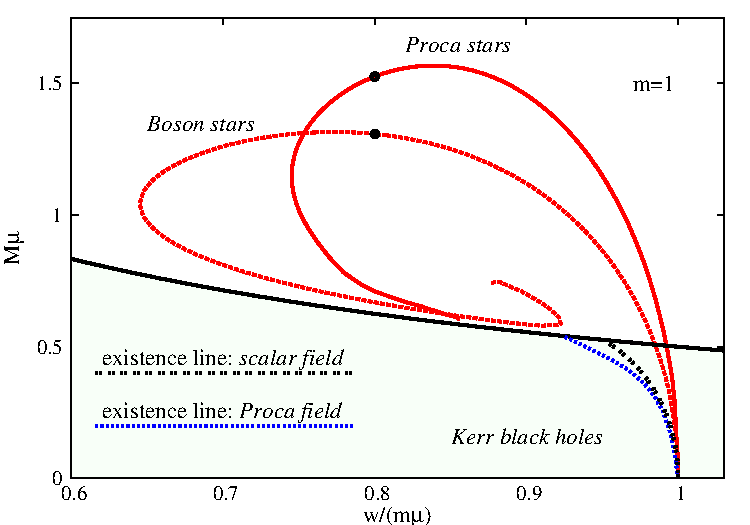
\includegraphics[width=0.7\textwidth]{papers/Proca/wM-m1-comparison.pdf}
  \end{center}
 \caption{Existence line for Proca stationary clouds with $m=1$ (blue dotted line) and the comparable existence line for scalar stationary clouds (with $m=1=\ell$, $n=0$, $cf.$~\cite{Benone:2014ssa}, black double dotted line), in an ADM mass $vs.$ frequency $w/m=\Omega_H$ diagram of Kerr BHs. Both axes are shown in units of the scalar/Proca field mass $\mu$. The black solid line corresponds to extremal Kerr BHs and non-extremal solutions exist below that line. Two red lines describing scalar boson stars (dotted) and Proca stars (solid) are also shown, that will be described in the next section.}
  \label{clouds}
\end{figure}

As can be seen from Fig. \ref{clouds}, there exist Kerr black holes that are superradiantly stable against all $m=1$ scalar perturbations but are superradiantly unstable against $m=1$ Proca modes.
A similar feature has been observed comparing the existence lines for \textit{Maxwell} and scalar stationary clouds in Kerr-AdS~\cite{Wang:2015fgp}.
As we saw in Chapter \ref{ch:Q}, including self-interactions in the scalar field model these stationary clouds can exist in open set of the $(M,\Omega_H)$ space, rather than a one-dimensional line.
We expect this to be the case as well if one would include self-interacting Proca fields, especially in view of the results in~\cite{Loginov:2015rya}.

We close this section by commenting on the node number of these stationary Proca clouds. 
In the scalar case, the number of nodes $n$ of the radial function defining the scalar field profile, 
is $n=0$ for fundamental states and $n\in \mathbb{N}$ for excited states. 
This issue becomes more subtle for Proca clouds (and Proca stars), 
since one has more than one potential component. Nevertheless, we remark that the all states we have obtained so far have always (only)
one node for the temporal component of the Proca potential  $V$, and thus are likely to represent the fundamental
modes of the problem.\footnote{The electric potential of the $m=0$ 
spherically symmetric Proca stars necessarily possesses at least one node \cite{Brito:2015pxa}.
Although the proof there cannot be generalized to the axially symmetric case,
we could not find any numerical indication for the existence of $m\geq 1$ nodeless solutions. 
}

%%%%%%%%%%%%%%%%%%%%%%%%%%%%%%%%%%%%%%%%%%%%%%%%%%%%%%%%%%%%%%%%%%%%%%%%%%%%%%
\section{Spinning Proca stars} 
\label{sec_stars}
%%%%%%%%%%%%%%%%%%%%%%%%%%%%%%%%%%%%%%%%%%%%%%%%%%%%%%%%%%%%%%%%%%%%%%%%%%%%%%
The stationary Proca clouds described in the previous section form one of the central ingredients to understand KBHsPH.
They also form a part of the boundary of the domain of existence of these BHs, as we shall see in the next section. The other central ingredient corresponds to Proca stars, which again will form a part of the boundary of the domain of existence of KBHsPH. We shall now briefly review the relevant properties of these solutions, recently found in~\cite{Brito:2015pxa}, for understanding KBHsPH.

Proca stars can be either spherically symmetric and static or axially symmetric and stationary. The former are found by taking a general spherically symmetric ansatz for the line element and an ansatz of the form $\mathcal{A}=e^{-iwt}\left[f(r)dt+ig(r)dr \right]$ for the Proca field.
With this ansatz, however, there are no BH solutions\cite{Herdeiro:2016tmi}. The latter are found by taking a metric ansatz of the form~\eqref{eqn:HBH-ansatz}, with $r_H=0$, with unspecified functions $F_0,F_1,F_2$ and the Proca potential ansatz~\eqref{procaclouds}, with unspecified functions $V,H_2,H_3$.
The remaining two (unspecified) functions are replaced as
\begin{equation}
W\rightarrow \frac{{W}}{r} \ , \qquad H_1\rightarrow \frac{{H_1}}{r} \ . 
\label{ww}
\end{equation}
We find it preferable to work with the new ${W},{H_1}$ when dealing with stars, due to their boundary conditions at the origin (rather than at a horizon). In the remaining of this section we shall always refer to these new functions.
Solving the corresponding field equations with the following boundary conditions:
\begin{description}
\item[i)] at infinity,~\eqref{bccloudslarge}, together with
\begin{equation}
F_i\big|_{r=\infty}={W}\big|_{r=\infty}=0 \ , 
\label{bcstarslarge}
\end{equation}
\item[ii)] on the symmetry axis,~\eqref{bccloudsaxis}, together with 
\begin{equation}
 \partial_\theta F_i\big|_{\theta=0,\pi}=\partial_\theta {W}\big|_{\theta=0,\pi}=0
 \label{bcstarsaxis}
 \end{equation}
 \item[iii)] at the origin, 
 \begin{equation}
 \partial_r F_i\big|_{r=0}={W}\big|_{r=0}=H_i|_{r=0}=V|_{r=0}=0 \ .
 \end{equation}
\end{description} 
 %
 Then, one finds a countable number of families of rotating Proca stars, labelled by $m\in \mathbb{Z}$, of which the cases with $m=1,2,3$ were discussed in~\cite{Brito:2015pxa}.  Therein, it was also found that, as for the scalar rotating boson stars, the ADM angular momentum and the Noether charge obey the simple relation 
 %
 \begin{equation}
 J=mQ \ .
\label{amnc}
 \end{equation}
%
In \cite{Herdeiro:2016tmi}, a detailed derivation and discussion of this relation is given, which is more subtle in the case of Proca stars than for scalar boson stars.
Following~\cite{Herdeiro:2014goa} and the discussion in Chapter \ref{ch:intro}, we define the normalized Noether charge, $q$, as 
 \begin{equation}
 q\equiv \frac{mQ}{J} \ ,
 \label{jq}
 \end{equation}
 which is obviously $q=1$ for all Proca stars, but will be $q\in (0,1]$ for KBHsPH.
 
 For $m=1$, the case in which we focus here, the Proca star solutions 
appear to form a spiral in an ADM mass, $M$, $vs.$ Proca field frequency, $w$, diagram, starting from $M=0$ for $w=\mu$, in which limit the Proca field becomes very diluted and the solution trivializes. 
At some intermediate frequency, a maximal ADM mass is attained. For $m=1$ this frequency is $w_{\rm max}/\mu=0.839$ and the maximal mass is $\mu M_{\rm max}=1.568$, a slightly larger value than for the corresponding scalar rotating boson star (for which $\mu M_{\rm max}=1.315$)~\cite{Brito:2015pxa}. 
 
In Fig.~\ref{clouds}, we display the $m=1$ Proca star and scalar boson star curves (red solid and dotted lines). Comparing them, we observe: $(i)$ the slightly larger maximal mass for the Proca stars; $(ii)$ that the backbending of the inspiraling curve occurs, for Proca stars, for a larger value of the frequency parameter, and hence they exist in a narrower frequency interval; $(iii)$ that whereas for scalar boson stars with $m=1$ it was possible to obtain a third branch of solutions (after the second backbending) numerics become very difficult for Proca stars already on the second branch;\footnote{In the spherically symmetric case, 
the results in \cite{Brito:2015pxa} show the existence of a very similar picture for both 
  Proca stars and scalar boson stars, with the occurance  of secondary branches (together with the corresponding
spiral in a $(w,M)$-diagram) also in the former case.} for example, 
the function $F_0$ takes very large, negative values.
Finally, in complete analogy with the scalar boson star case, the Proca star line yields the second boundary of the domain of existence of KBHsPH; the latter reduce to Proca stars when the horizon size vanishes, as will be seen in the next section. 

Although spinning Proca stars are quite similar to spinning scalar boson stars in many aspects, the energy and angular momentum density of the former exhibit novel features with respect to the latter.
Spinning scalar boson stars for generic $m\geqslant 1$ are often described as an effective mass torus in general relativity~\cite{Schunck:1996he}, since surfaces of constant energy density present a toroidal topology sufficiently close to the centre of the star (see $e.g.$ the plots in~\cite{Herdeiro:2014ima}).
Spinning Proca stars, on the other hand, have a different structure for $m=1$ and $m>1$ as shown in Figs.~\ref{PS1}--\ref{3D} for illustrative cases (with $w=0.8$ and along the first branch for all examples).
For $m=1$, the Proca star's energy density has a maximum at the origin and a second maximum (smaller) at some radial distance, thus presenting a composite-like structure, $cf.$ Fig.~\ref{PS1} (top left panel): instead of being toroidal some constant energy surfaces are \textit{Saturn-like} - Fig.~\ref{3D} (left panel).
The angular momentum density, on the other hand, is zero at the origin and has two local positive maxima at some radii and one local negative minimum between them -- Fig.~\ref{PS1} (top right panel); in particular this means there is a counter-rotating toroidal-like region.
For $m>1$ the Proca star's energy density vanishes at the origin and two local maxima arise at different radial values, $cf.$ Fig.~\ref{PS2} (top left panel).
Thus some constant energy density surfaces are \textit{di-ring-like} - Fig.~\ref{3D} (right panel).
The angular momentum density is similar to the $m=1$ case -- Fig.~\ref{PS2} (top right panel).


\begin{figure}[h!]
  \begin{center}
    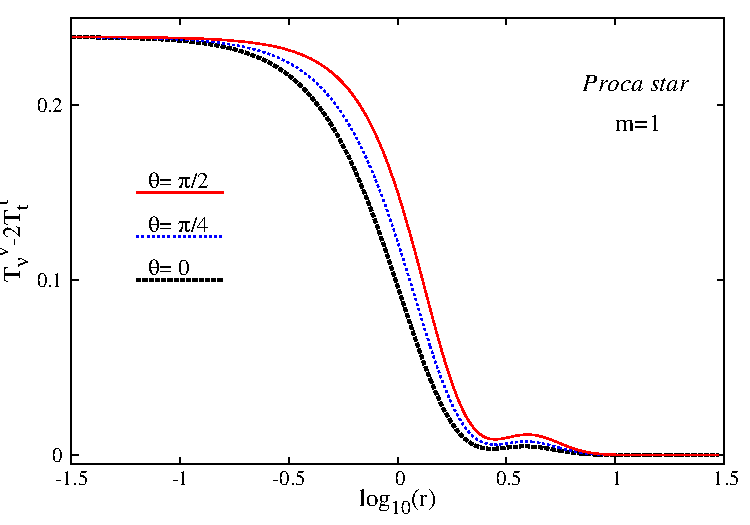
\includegraphics[width=8.1cm]{papers/Proca/PS-ro-m1.pdf}
    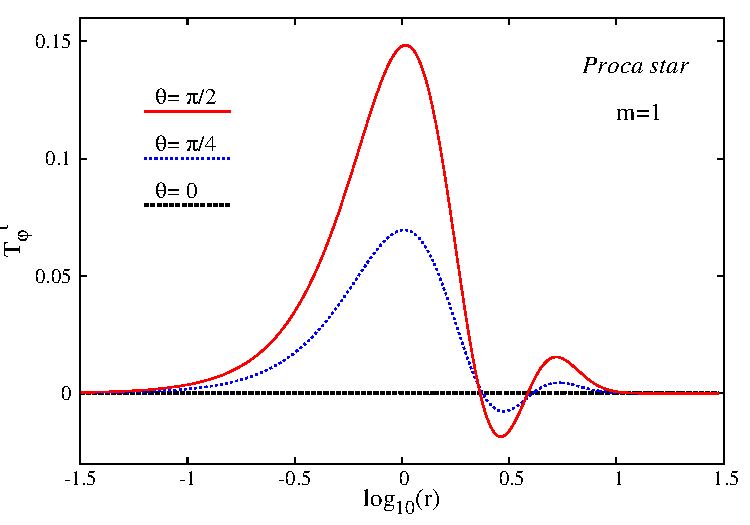
\includegraphics[width=8.1cm]{papers/Proca/PS-T34-m1.pdf}   
    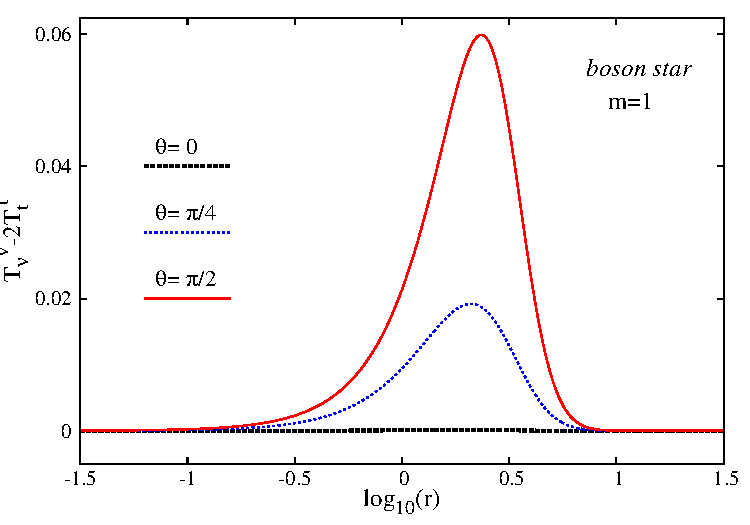
\includegraphics[width=8.1cm]{papers/Proca/BS-ro-m1.pdf}
    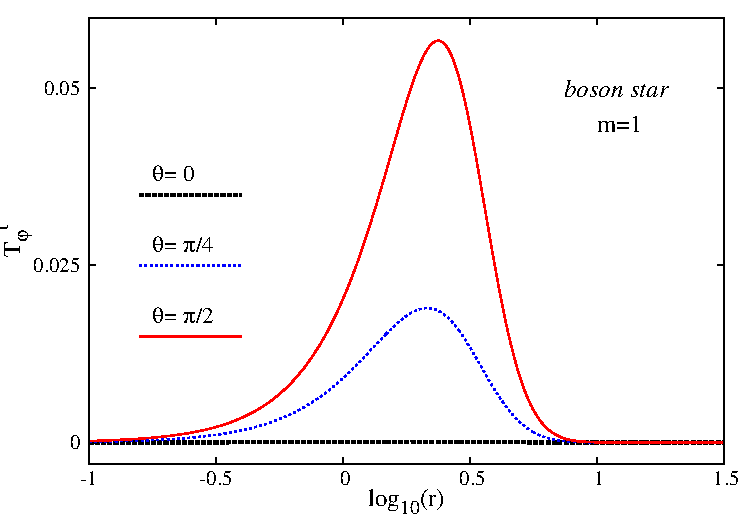
\includegraphics[width=8.1cm]{papers/Proca/BS-T34-m1.pdf}
  \end{center}
 \caption{Radial variation of the energy density, $cf.$~\eqref{ed} (left panel), and angular momentum density, $cf.$~\eqref{amd}  (right panel),  of the Proca field, for different constant $\theta$ sections of a spinning Proca star with $m=1$ (top panels) and a spinning scalar boson star with $m=1$ (bottom panels). Both solutions have $w=0.8$ and are marked with a bullet in Fig.~\ref{clouds}. The Proca star has $\mu M= 1.526$,  $\mu^2J= 1.575$, while the scalar boson star has $\mu M=1.308$, $\mu^2J=1.372$.}
  \label{PS1}
\end{figure}



\begin{figure}[h!]
  \begin{center}
    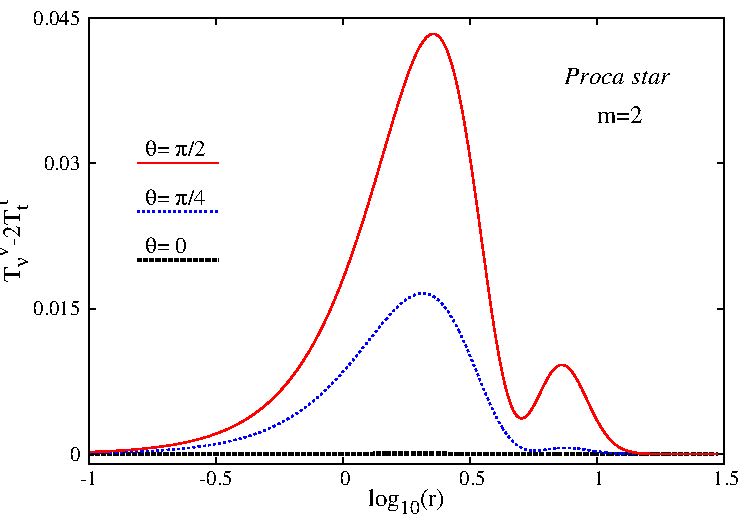
\includegraphics[width=8.1cm]{papers/Proca/PS-ro-m2.pdf}
    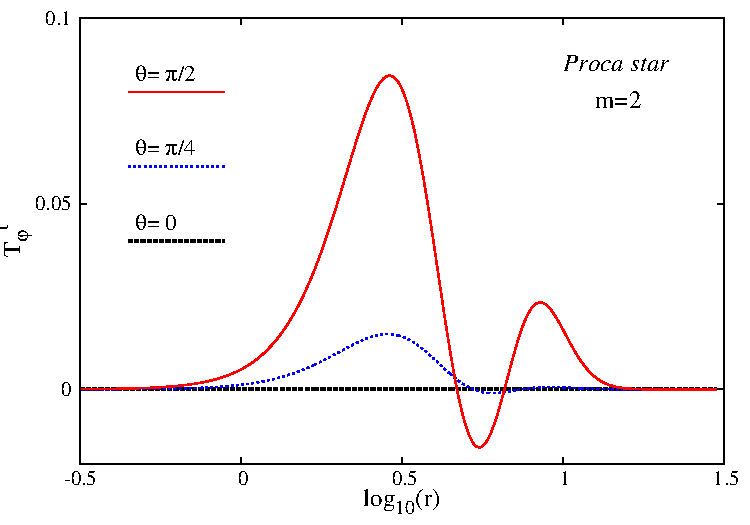
\includegraphics[width=8.1cm]{papers/Proca/PS-T34-m2.pdf}   
    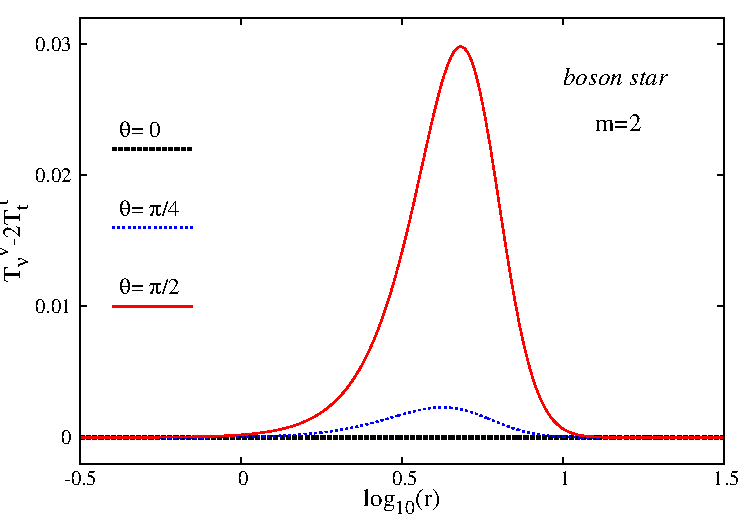
\includegraphics[width=8.1cm]{papers/Proca/BS-ro-m2.pdf}
    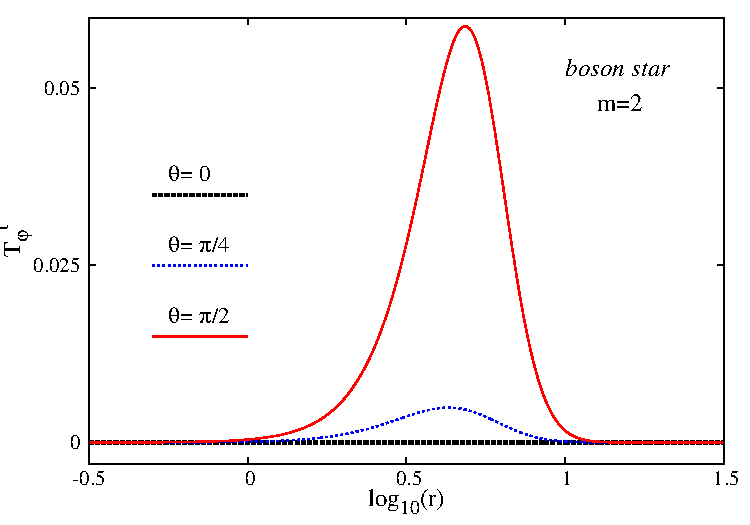
\includegraphics[width=8.1cm]{papers/Proca/BS-T34-m2.pdf}
  \end{center}
 \caption{Same as in Fig.~\ref{PS1} but for $m=2$. Both solutions have $w=0.8$. The Proca star has $\mu M=2.319$, 
$\mu^2J=4.873$ whereas the scalar boson star has $\mu M=2.016$, $\mu^2J=4.272$.}
  \label{PS2}
\end{figure}


\begin{figure}[h!]
  \begin{center}
    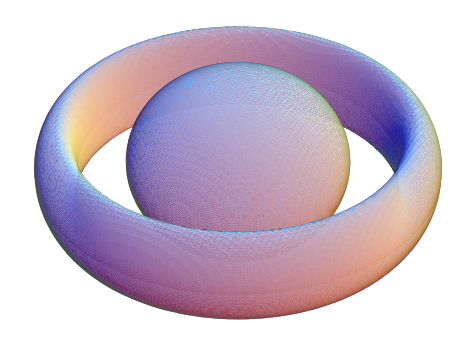
\includegraphics[width=6.1cm]{papers/Proca/3DPS1-m=1-v2.pdf} \qquad \qquad 
    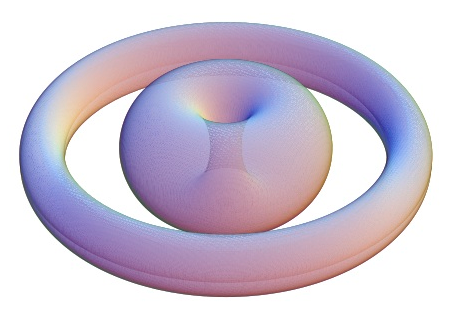
\includegraphics[width=6.1cm]{papers/Proca/3DPS1-m=2-v2.pdf}   
         \end{center}
 \caption{Left (right) panel: Saturn-like (di-ring-like) surfaces of constant energy density for the $m=1$ ($m=2$) Proca star exhibited in Fig.~\ref{PS1} (Fig.~\ref{PS2}). The corresponding energy density is $0.011$ ($0.008$). We emphasize these are not embedding diagrams; rather we defined Cartesian coordinates regarding the $r,\theta,\varphi$ coordinate system used here as standard spherical coordinates.}
  \label{3D}
\end{figure}

Finally, we discuss how ``compact'' these Proca stars are.
Proca stars, like their scalar cousins, have no surface, $i.e.$ the Proca field decays exponentially towards infinity.
Thus, there is no unique definition of the Proca star's ``radius''.
To obtain an estimate we follow the discussion in~\cite{AmaroSeoane:2010qx,Herdeiro:2015gia}.
Using the ``perimeteral'' radius, $i.e.$, a radial coordinate $R$ such that a circumference along the equatorial plane has perimeter $\simeq 2\pi R$,  we compute $R_{99}$, the perimeteral radius containing 99\% of the Proca star mass, $M_{99}$. Then, we define the inverse compactness by comparing $R_{99}$ with the Schwarzschild radius associated to 99\% of the Proca star's mass, $R_{Schw}=2M_{99}$:
%
\begin{equation}
{\rm Compactness}^{-1}\equiv  \frac{R_{99}}{2M_{99}} \ .
\label{compactness}
\end{equation}
%
The result for the inverse compactness of Proca stars with $m=1$ is exhibited in Figure~\ref{compactnessfig}.
With this measure, the inverse compactness is always greater than unity; $i.e.$, Proca stars are less compact than BHs, as one would expect, but they are also less compact than comparable scalar boson stars.

\begin{figure}[h!]
  \begin{center}
    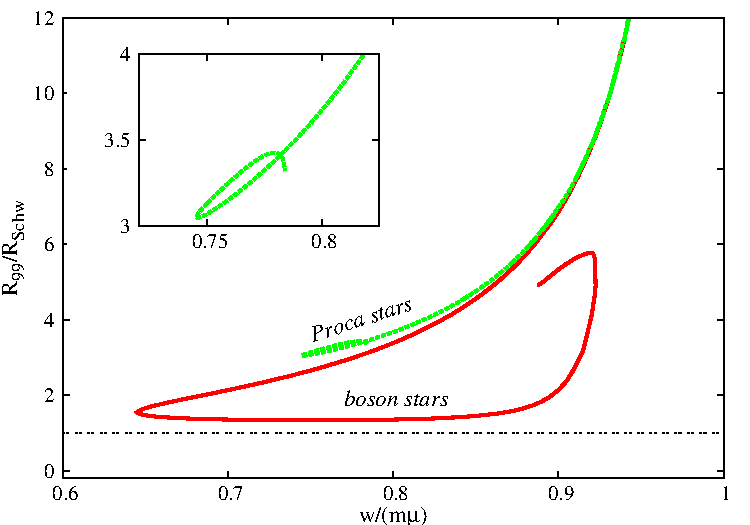
\includegraphics[width=0.7\textwidth]{papers/Proca/w-Comp-Schw.pdf}  
         \end{center}
 \caption{Inverse compactness of Proca stars compared to that of the scalar boson stars with $m=1$, defined in~\eqref{compactness}. The inset shows a detail of the Proca stars curve.}
  \label{compactnessfig}
\end{figure}

%%%%%%%%%%%%%%%%%%%%%%%%%%%%%%%%%%%%%%%%%%%%%%%%%%%%%%%%%%%%%%%%%%%%%%%%%%%%%%
\section{Kerr BHs with Proca Hair} 
\label{sec_kbhsph}
%%%%%%%%%%%%%%%%%%%%%%%%%%%%%%%%%%%%%%%%%%%%%%%%%%%%%%%%%%%%%%%%%%%%%%%%%%%%%%

We are now prepared to take on KBHsPH.
The parallelism with the scalar case for both the stationary clouds and the solitonic limit is striking and one anticipates a high degree of similarity also at the level of the hairy BH solutions. 

The metric ansatz for constructing KBHsPH is the same as for the previous examples of hairy black holes, i.e. Eq.~\eqref{eqn:HBH-ansatz}, where now all four (unspecified) functions $F_0,F_1,F_2,W$ depend on $(r,\theta)$ and, again, $r_H$ is a constant.
If $F_2$ is finite, then $r={\rm constant}$ surfaces are timelike for $r>r_H$ and become null for $r=r_H$.
Thus, $r=r_H$ is the location of the event horizon if the metric is regular therein.

For $r_H=0$, this ansatz reduces to the one discussed in the previous section for Proca stars, except for the replacement given by Eq.~\eqref{ww}.
The line element form used for Proca stars is useful to tackle the behaviour at the origin, whereas the one used for BHs is useful to tackle the behaviour on a rotating horizon wherein $W$ reduces to the horizon angular velocity, $\Omega_H$.
Indeed, following null geodesic generators ($ds^2=0$) on the horizon ($r=r_H$), assuming $F_2$ is finite therein, implies $d\varphi=W(r_H)dt$ and thus $W(r_H)=\Omega_H$, the angular velocity as measured by the observer at infinity.

The Proca field ansatz is the same as for the stationary Proca clouds (and Proca stars up to the replacements given by Eq.~\eqref{ww}),given by Eq.~\eqref{procaclouds}.
This, again, introduces two parameters: $w>0$, $m\in \mathbb{Z}$.
As for Proca stars we shall focus here on $m=1$, and take the sychronization condition~\eqref{synchronization} that we can rewrite in this context as (for general $m$)
\begin{equation}
\frac{w}{m}=W(r_H) =\Omega_H\ . 
\label{synchronization2}
\end{equation}
This condition was deduced in the context of a test field on the Kerr background and can be related to the threshold of superradiance.
But there is another reason for its presence.
In Appendix~\ref{appendixb}, we present the Einstein tensor and the Proca energy-momentum tensor associated to the ansatz discussed in this section.
A careful inspection of the components of the energy-momentum tensor that have inverse powers of $N$,\footnote{A similar analysis can be made at the level of the components in an orthonormal frame, with similar conclusions.} and hence may diverge at the horizon, shows that, taking into account Eq.~\eqref{bccloudshorizon}, finiteness of the energy-momentum tensor components presented at $r=r_H$ \textit{requires}
\begin{equation}
\frac{w-mW(r_H)}{N(r_H)} 
\end{equation}
to be finite and hence it requires Eq.~\eqref{synchronization2} to be fulfilled.
The same can be observed in the Einstein equations for KBHsSH, presented in~\cite{Herdeiro:2015gia}.
It is interesting to remark that this finiteness condition, i.e. Eq.~\eqref{synchronization2}, is not necessarily related to superradiance, as the higher dimensional examples in~\cite{Brihaye:2014nba,Herdeiro:2015kha} illustrate. 


The Einstein-Proca equations are solved with the following boundary conditions (which again we have found to be compatible with an approximate construction of the solutions
on the boundary of the domain of integration):  
\begin{description}
\item[i)] at infinity, the same as for Proca stars,~\eqref{bccloudslarge} and~\eqref{bcstarslarge};
\item[ii)] on the symmetry axis, the same as for Proca stars,~\eqref{bccloudsaxis} and~\eqref{bcstarsaxis};
 
\item[iii)] at the horizon, using again the new radial coordinate $x=\sqrt{r^2-r_H^2}$, a power series expansion near $x=0$ implies~\eqref{bccloudshorizon}, together with
\begin{equation}
\partial_x F_i\big|_{x=0}=0 \ , \qquad W\big|_{x=0}=\Omega_H \ .
\end{equation}
\end{description}
 % 

The Einstein-Proca equations,shown in Appendix \ref{appendixb}), are solved numerically subject to these boundary conditions.


%%%%%%%%%%%%%%%%%%%%%%%%%%%%%%%%%%%%%%%%%%%%%%%%%%%%%%%%%%%%%%%%%%%%%%%%%%%%%%%
\subsection{Physical Quantities}
\label{subsec_II}
%%%%%%%%%%%%%%%%%%%%%%%%%%%%%%%%%%%%%%%%%%%%%%%%%%%%%%%%%%%%%%%%%%%%%%%%%%%%%%% 
In the following we shall describe some physical quantities that will be monitored from the numerical solutions we have obtained.
The ADM mass, $M$, and ADM angular momentum, $J$, are read off from the asymptotic expansion of the appropriate metric components:
%
\begin{equation}
\label{Pasym}
g_{tt} =-1+\frac{2M}{r}+\dots \ ,\qquad ~~g_{\varphi t}=-\frac{2J}{r}\sin^2\theta+\dots \ . \ \ \ 
\end{equation}
%
We also compute the horizon mass and angular momentum by using the appropriate Komar integrals associated to the corresponding Killing vector fields ${\bf k}$ and ${\bf m}$:
\begin{equation}
M_H=-\frac{1}{8\pi}\oint_{\mathcal{H}}dS_{\alpha\beta}D^\alpha k^\beta \ , \qquad 
J_H=\frac{1}{16\pi}\oint_{\mathcal{H}}dS_{\alpha\beta}D^\alpha m^\beta \ .
\end{equation}
%
Both $M$ and $J$ can also be computed as Komar integrals at infinity.
Then, applying Gauss's law, one obtains a relation with $M_H$ and $J_H$ together with volume integrals on a spacelike surface with a boundary at the (spatial section of the) horizon.
By making use of the Killing identity and the Einstein equations one obtains:
\begin{equation}
M=M_H-2\int_{\Sigma}dS_{\alpha}\left(T^\alpha_\beta k^\beta-\frac{1}{2}Tk^\alpha\right) \equiv M_H+M^{(\mathcal{P})}
\end{equation}
This defines the energy stored in the Proca field (outside the horizon):
\begin{equation}
M^{({\cal P})}\equiv - \int_{\Sigma} dr d\theta d\varphi(2T_t^t-T_\alpha^\alpha) \sqrt{-g} \ .
\label{ed}
\end{equation}
%
Proceeding similarly for the angular momentum one obtains:
\begin{equation}
J=J_H+J^{(\mathcal{P})} \ , \ \qquad  J^{({\cal P})}\equiv  \int_{\Sigma} dr d\theta d\varphi T^t_\varphi \sqrt{-g} \ ,
\label{amd}
\end{equation}
which defines the angular momentum stored in the Proca field.
For KBHsSH the angular momentum stored in the scalar field relates to the Noether charge in precisely the same way as for rotating scalar boson stars $J^{(\Psi)}=mQ$, for KBHsPH the relation between $J^{(\mathcal{P})} $ and  the Noether charge~\eqref{Pq} includes an extra boundary term
\begin{equation}
\label{nr1}
J^{(\mathcal{P})}=mQ+ \oint_\mathcal{H}  ({\mathcal{A}}_\varphi \bar{ {\mathcal{F}}}^{r t}+\bar{\mathcal{A}}_\varphi { {\mathcal{F}}}^{r t}  ) dS_r \ ,
\end{equation}
which generalizes relation~\eqref{amnc} to the case of hairy BHs. 
A similar relation can be written for $M^{({\cal P})}$
\begin{equation}
\label{nr2}
M^{({\cal P})}=2w Q
-\mu^2  {\cal U}
+ \oint_\mathcal{H}  
\left[
\frac{1}{2} 
\left(
{\mathcal{A}}_\beta \bar{ {\mathcal{F}}}^{r \beta}+\bar{\mathcal{A}}_\beta { {\mathcal{F}}}^{r \beta}
\right)
-\left({\mathcal{A}}_t \bar{ {\mathcal{F}}}^{r t}+\bar{\mathcal{A}}_t { {\mathcal{F}}}^{r t}
\right)  
\right] dS_r \ ,
\end{equation}
with
\begin{equation}
\label{ProcaU}
{\cal U}\equiv \int _\Sigma  dr d\theta d\varphi  {\mathcal{A}}_\alpha \bar {\mathcal{A}}^\alpha \sqrt{-g}\ .
\end{equation}


The horizon temperature and event horizon area of the KBHsPH solutions are computed by standard relations, that specialize to: 
\begin{eqnarray}
\label{PTHAH}
T_H=\frac{1}{4\pi r_H}e^{(F_0-F_1)|_{r=r_H}} \ , \qquad
 A_H=2\pi r_H^2 \int_0^\pi d\theta \sin \theta  e^{(F_1+F_2)|_{r=r_H}}\ . 
 \end{eqnarray}
Then, the ADM quantities $M,J$ are related with $T_H,S,Q,M^{({\cal P})}$, where $S=A_H/4$ is the horizon entropy, through a Smarr formula  
%
\begin{eqnarray}
\label{Psmarr} 
M=2 T_H S +2\Omega_H J_H+ M^{({\cal P})} \ .
\end{eqnarray}
The variation of $M$ can be expressed by the first law
\begin{equation}
\label{fl}
dM=T_H dS +\Omega_H dJ \ .
\end{equation}
We note that
by making use of relations
(\ref{nr1})
and
(\ref{nr2}),
 the Smarr formula (\ref{Psmarr})
can be written in a Kerr-like form
\begin{eqnarray}
\label{smarr-new1} 
M=2 T_H S +2\Omega_H J-\mu^2 {\cal U} \ ,
\end{eqnarray}
which renders explicit the fact that the solutions are supported by
a nonzero mass term of the Proca field.

Finally, we observe that Proca stars
satisfy a simple relation, which results again from relations (\ref{nr1}) and (\ref{nr2}):\footnote{One can similarly show that KBHsSH and scalar boson stars satisfy relations analogous to
(\ref{smarr-new1}) and  (\ref{smarr-new2}), respectively.} 
\begin{eqnarray}
\label{smarr-new2} 
M=2 w Q-\mu^2 {\cal U}=2\frac{w}{m} J-\mu^2 {\cal U}\ .
\end{eqnarray}

%%%%%%%%%%%%%%%%%%%%%%%%%%%%%%%%%%%%%%%%%%%%%%%%%%%%%%%%%%%%%%%%%%%%%%%%%%%%%%%
\subsection{The domain of existence and phase space}
\label{subsec_III}
%%%%%%%%%%%%%%%%%%%%%%%%%%%%%%%%%%%%%%%%%%%%%%%%%%%%%%%%%%%%%%%%%%%%%%%%%%%%%%% 
We have scanned the domain of existence of KBHsPH by varying $r_H$ for fixed $w$ lines, 
in between the minimum frequency 
$w_{\rm min}/\mu=0.7453$ and the maximal one $w=\mu$. 
The result for the $m=1$ family of KBHsPH is shown in Fig.~\ref{figdomain} obtained from over five thousand numerical points. 


%
\begin{figure}[h!]
  \begin{center}
    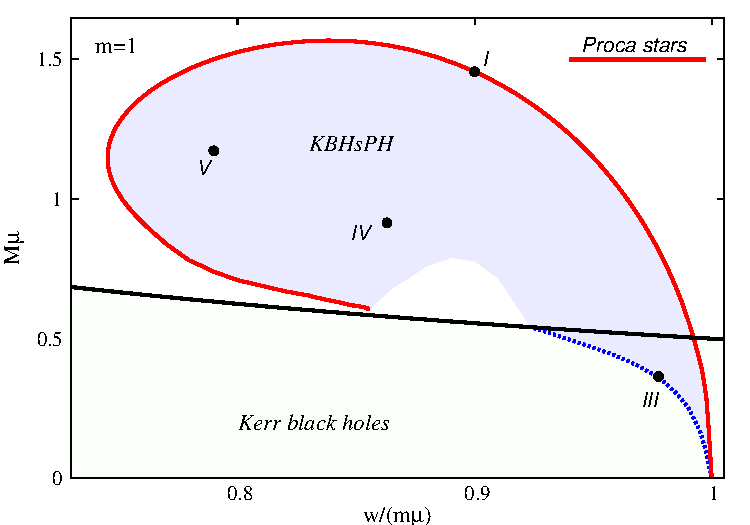
\includegraphics[width=0.7\textwidth]{papers/Proca/BH-w-M-with-points.pdf}
      % 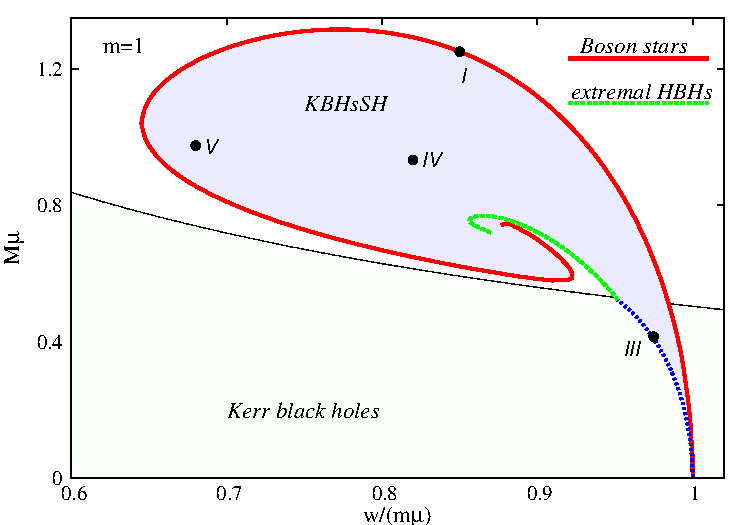
\includegraphics[width=8.1cm]{papers/Proca/scalar-BH-w-M.pdf}
  \end{center}
  \caption{ADM mass $vs.$ frequency $w$ diagram for $m=1$ KBHsPH. The red solid lines correspond to the solitonic limit. The blue dotted lines are the Kerr limit, also shown in Fig.~\ref{clouds}. Kerr solutions exist below the black solid line, which corresponds to extremal Kerr solutions. The hairy BHs exist in the blue shaded region. Points I,III,IV,V, in each case, correspond to specific solutions for which the numerical data is publicly available~\cite{datakbhph,datakbhsh}. The right panel also shows the extremal hairy BHs (green dashed) line.}
  \label{figdomain}
\end{figure}
%


Based on the discussions of KBHsSH~\cite{Herdeiro:2014goa,Herdeiro:2015gia,Herdeiro:2015tia}, and as already partly discussed, the domain of existence of KBHsPH should be bounded by three lines: the Proca clouds existence line discussed in Section~\ref{sec_clouds}, the Proca star line discussed in Section~\ref{sec_stars} and the line of extremal KBHsPH ($i.e.$ zero temperature).
So far, the last of the three were only obtained by extrapolating to $T_H=0$ the non-extremal solutions, as our attempts to construct the extremal KBHsPH solutions by directly solving the Einstein-Proca field equations were unsuccessful (unlike the scalar case, as reported in~\cite{Herdeiro:2015gia} and Chapter \ref{ch:SI} for self-interacting solutions).
For this reason we have chosen not to display this line in Fig.~\ref{figdomain}, for the Proca case.
Another technical difficulty arises in trying to connect the set of (extrapolated) extremal solutions with the set of Proca stars.
As for the case of KBHsSH, these two curves are likely to meet in a critical point at the center of the 
Proca stars spiral; however, validation of this hypothesis is a numerical challenge, both for the Proca and scalar case.

In Fig.~\ref{figdomain} we have singled out four particular solutions for each case, denoted I,III,IV and V. The numerical data for these four solutions, together with the data for a vacuum Kerr solution with the same ADM mass and angular momentum as that of configuration III, for each case, has been made publicly available for community use~\cite{datakbhph,datakbhsh}. The corresponding parameters are detailed in Appendix~\ref{appendixd}.

In Fig.~\ref{fig2} we exhibit the phase space, $i.e.$ ADM mass $vs.$ ADM angular momentum diagram for $m=1$ solutions of KBHsPH.
The plot is quite similar to the top left panel of Fig.~\ref{fig:no-HBHs} and the features we wish to emphasize is that, as for the scalar case, one observes violation of the Kerr bound (in terms of ADM quantities) and non-uniqueness, $i.e$ there are both hairy and vacuum Kerr BHs with the same ADM mass and angular momentum ($cf.$ Appendix~\ref{appendixd}). 


\begin{figure}[h!]
  \begin{center}
    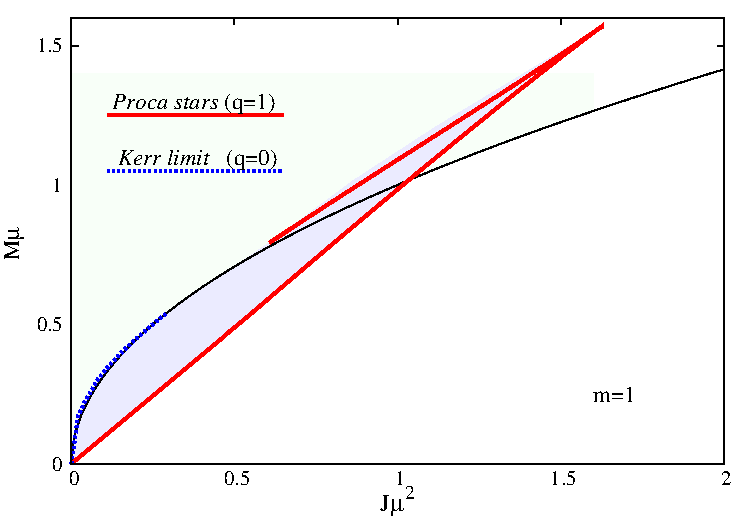
\includegraphics[width=0.7\textwidth]{papers/Proca/BH-J-M.pdf}
  \end{center}
  \caption{ADM mass $vs.$ ADM angular momentum diagram for $m=1$ KBHsPH, in units of the field mass. The black solid line corresponds to extremal Kerr solutions; non extremal BHs exist above this line. The red solid line is for Proca stars in the left panel. The blued dotted line is the existence line, denoting Kerr BHs that support Proca clouds. The blue shaded region is the domain of existence of KBHsPH.}
  \label{fig2}
\end{figure}
 

The violation of the Kerr bound also occurs in terms of \textit{horizon} quantities, as shown in Fig.~\ref{vconjecture} (right panel). For these solutions the conjecture put forward in~\cite{Herdeiro:2015moa} concerning the horizon linear velocity $v_H$, as defined therein, holds: despite violating the Kerr bound both in terms of ADM and horizon quantities, $v_H$ never exceeds the speed of light.  We recall $v_H$ is defined as follows, for asymptotically flat, stationary and axi-symmetric spacetimes. On a spatial section of the event horizon one computes the proper length of all closed orbits of ${\bf m}$. Let $L_{\rm max}$ be the maximum of all such proper lengths; the corresponding circumferencial radius, $R_c$, is $R_c\equiv {L_{\rm max}}/({2\pi})$. 
The horizon linear velocity is $v_H \equiv R_c \Omega_H$ \cite{Herdeiro:2015moa}.

\begin{figure}[h!]
  \begin{center}
    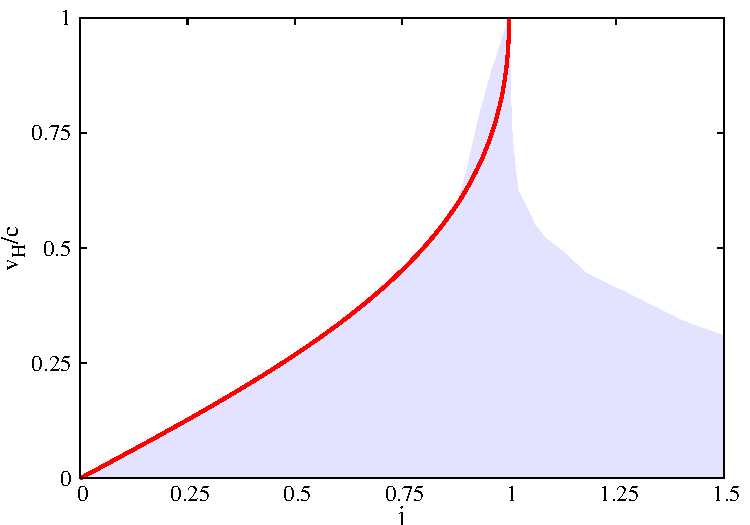
\includegraphics[width=8.1cm]{papers/Proca/ProcaBH-j-v-bound.pdf}
      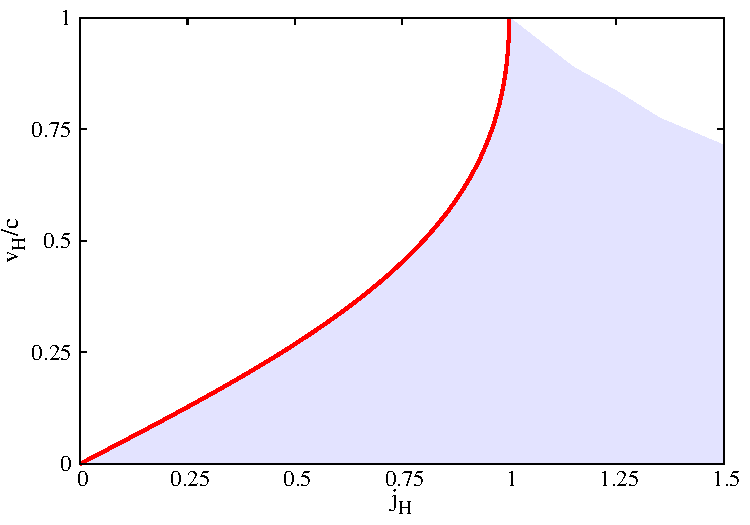
\includegraphics[width=8.1cm]{papers/Proca/ProcaBH-jKv-bound.pdf}
  \end{center}
 \caption{Linear velocity of the horizon normalized to the speed of light, $v_H$, versus:  (left panel)  the ADM dimensionless spin parameter $j\equiv Jc/GM^2$, where $M,J$ are the ADM mass and angular momentum; (right panel) the horizon dimensionless spin parameter $j_H\equiv J_Hc/GM_H^2$, where $M_H,J_H$ are the horizon mass and angular momentum. Here we have reinstated $c,G$. The red solid line corresponds to vacuum Kerr and the shaded area is filled by KBHsPH.}
  \label{vconjecture}
\end{figure}

%%%%%%%%%%%%%%%%%%%%%%%%%%%%%%%%%%%%%%%%%%%%%%%%%%%%%%%%%%%%%%%%%%%%%%%%%%%%%%%
\subsection{Energy distribution and horizon quantities}
\label{subsec_IV}
%%%%%%%%%%%%%%%%%%%%%%%%%%%%%%%%%%%%%%%%%%%%%%%%%%%%%%%%%%%%%%%%%%%%%%%%%%%%%%%
As for their scalar counterparts, KBHsPH can be thought of as a bound state of a horizon with a Proca star.
Thus, the matter energy density distribution around the horizon will resemble that of (some) Proca stars.
In~Fig.~\ref{figenergybhs} we exhibit the energy density and the angular momentum density as a function of the radial coordinate for different angular sections for an example of KBHPH.
As for the Proca stars, both the energy density and the angular momentum density can have more than one maximum outside the horizon and the latter can also have regions with a different sign.
Thus, outside KBHsPH there are counter-rotating regions.
In Fig.~\ref{fig3Dbh} a constant Proca energy density surface is exhbited in a 3D plot.
The behaviour of the energy density and angular momentum density on the horizon is more clearly seen in Fig.~\ref{horizoned}.


\begin{figure}[h!]
  \begin{center}
    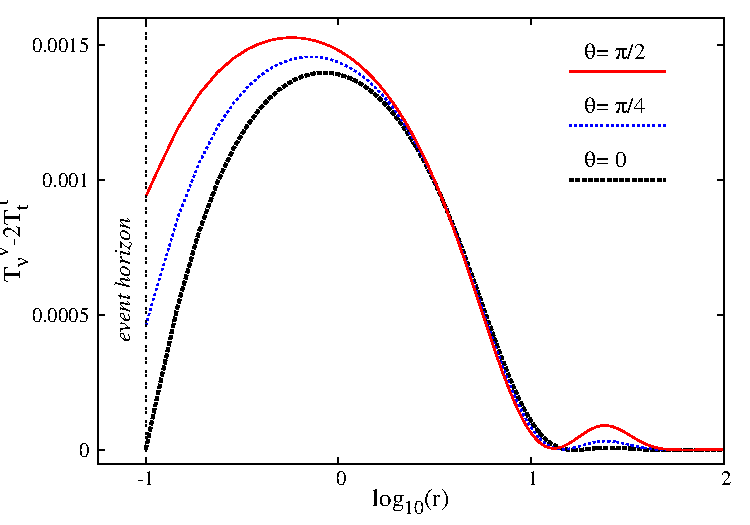
\includegraphics[width=8.1cm]{papers/Proca/BH-ro-m1.pdf}
      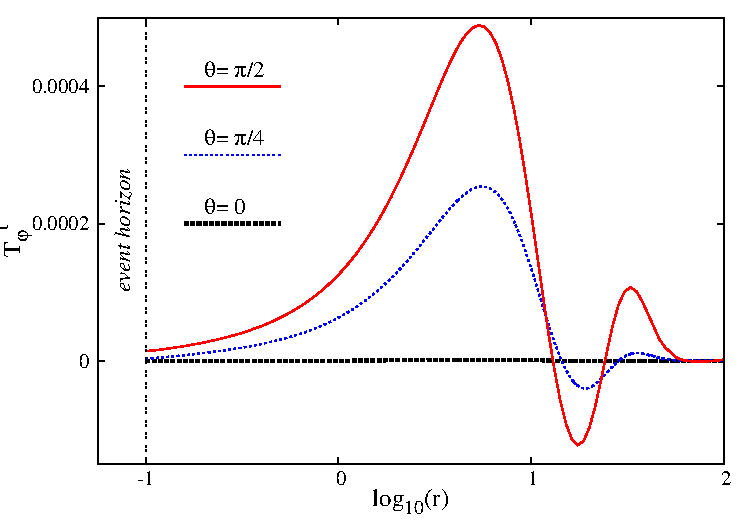
\includegraphics[width=8.1cm]{papers/Proca/BH-T34.pdf}
  \end{center}
  \caption{Radial variation of the energy density, $cf.$~\eqref{ed} (left panel), and angular momentum density, $cf.$~\eqref{amd}  (right panel),  of the Proca field, for different constant $\theta$ sections of a KBHPH with $m=1$, $w=0.98\mu$, $r_H=0.1$,  $\mu M=0.701$ and $\mu^2J=0.652$.}
  \label{figenergybhs}
\end{figure}



\begin{figure}[h!]
  \begin{center}
    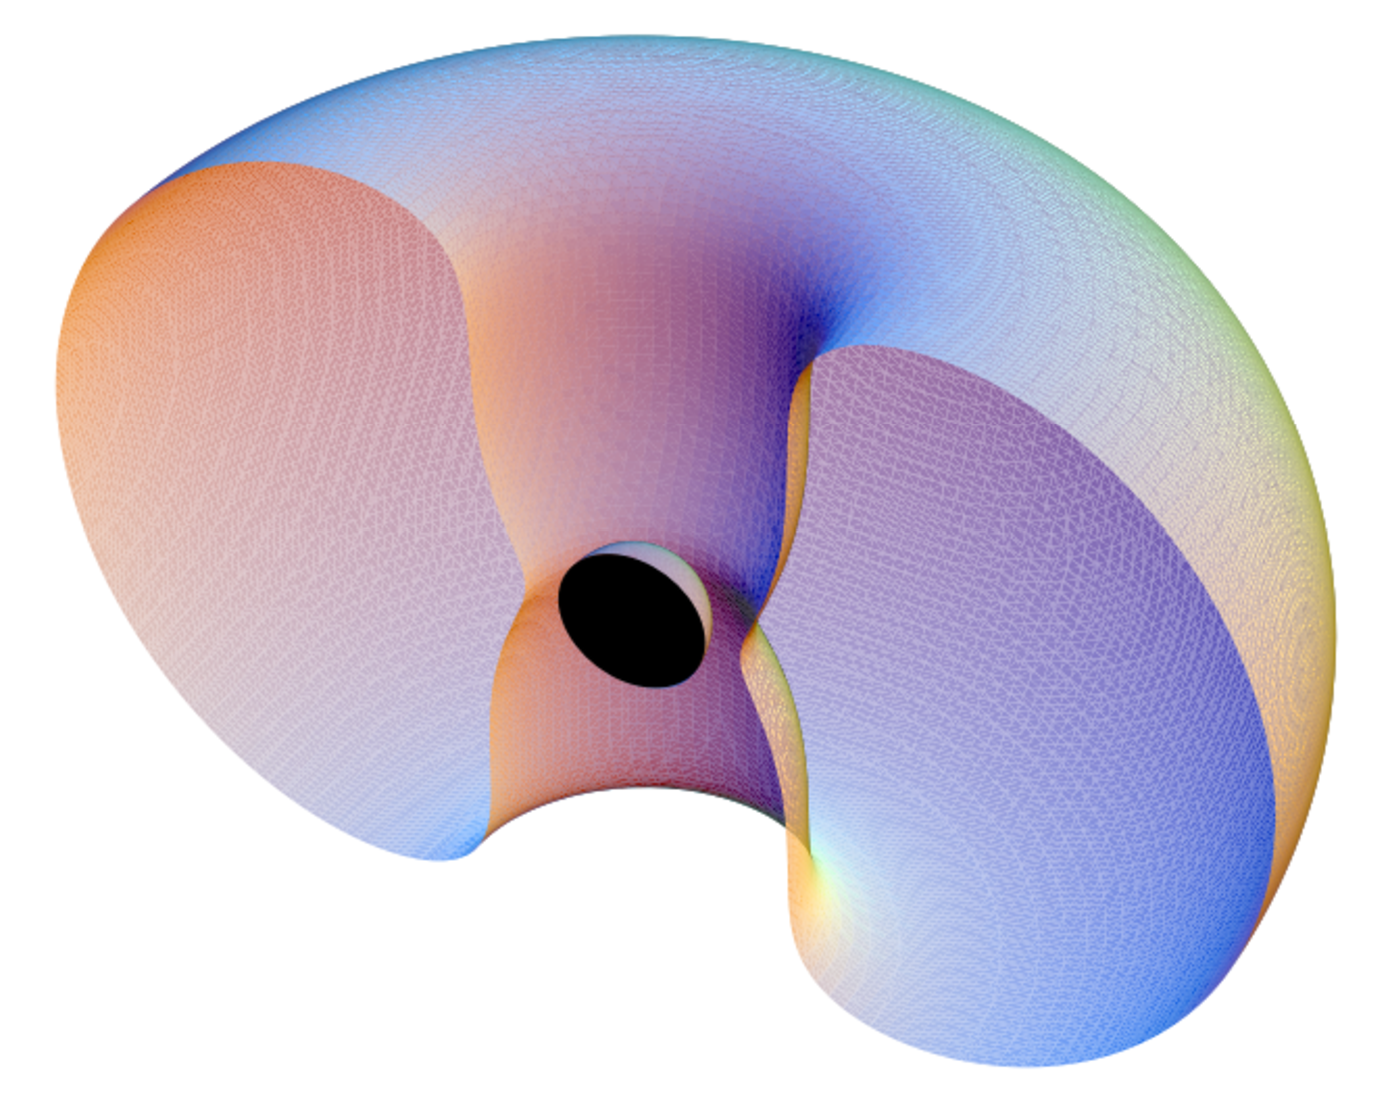
\includegraphics[width=6.1cm]{papers/Proca/3Dbh.pdf}
  \end{center}
  \caption{One toroidal-like surface of constant energy density (corresponding to $0.00142$) for the same KBHPH displayed in Fig.~\ref{figenergybhs}. We also plot the spatial section of the event horizon in these coordinates (half-sphere with the black cross section).}
  \label{fig3Dbh}
\end{figure}


\begin{figure}[h!]
  \begin{center}
    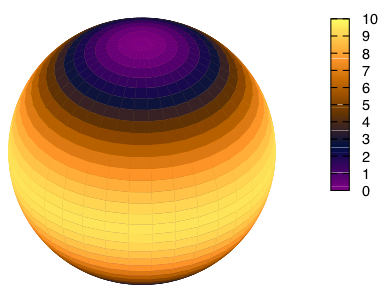
\includegraphics[width=5.5cm]{papers/Proca/Ttr-horizon.pdf}\qquad \qquad 
      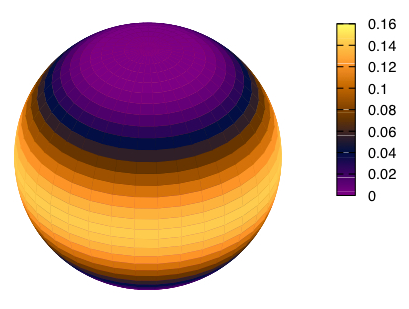
\includegraphics[width=6.0cm]{papers/Proca/T34-horizon.pdf}
  \end{center}
  \caption{Energy density, $cf.$~\eqref{ed} (left panel), and angular momentum density, $cf.$~\eqref{amd}  (right panel),  of the Proca field on the horizon for the same example of a KBHPH displayed in Fig.~\ref{figenergybhs}. The corresponding values were multiplied by $10^4$ for better visualization.}
  \label{horizoned}
\end{figure}


Finally, in Fig.~\ref{temperature} we exhibit the variation of the horizon area with the horizon temperature along sequences of solutions with constant horizon angular velocity (or frequency).
For both KBHsPH (left panel) and KBHsSH (right panel) one can see three different types of behaviour, which are easy to interpret referring back to Fig.~\ref{figdomain}.
For large values of $\Omega_H$, the solutions interpolate between the Kerr existence line and the corresponding (Proca or scalar boson) star line (for which $T_H\rightarrow \infty$).
For intermediate values of $\Omega_H$, the solutions interpolate between the extremal BHs line (for which $T_H\rightarrow 0$) and the corresponding star line.
Finally, for sufficiently small values of $\Omega_H$, the solutions interpolate between two stars, and thus start and end for $T_H\rightarrow \infty$.


\begin{figure}[h!]
  \begin{center}
    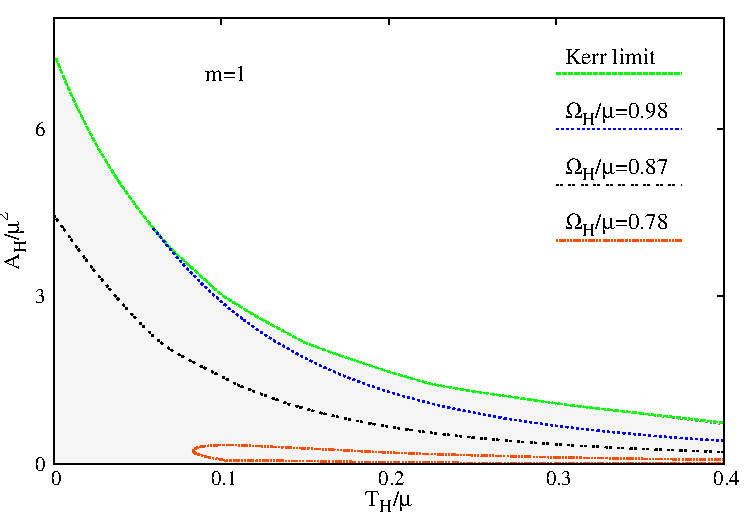
\includegraphics[width=8.1cm]{papers/Proca/BH-TH-AH.pdf}
      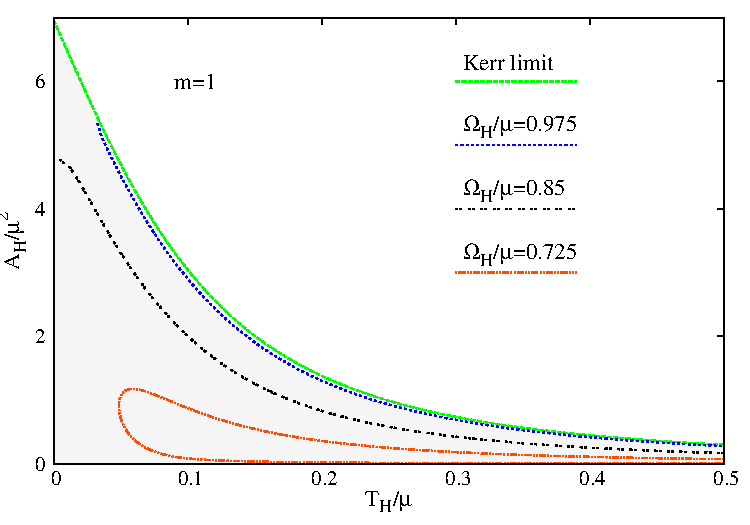
\includegraphics[width=8.1cm]{papers/Proca/scalar-BH-TH-AH.pdf}
  \end{center}
 \caption{Event horizon area $vs.$ temperature for KBHsPH (left panel) and KBHsSH (right panel), in units of $\mu$, for different constant angular velocity sets of solutions.}
  \label{temperature}
\end{figure}
%%%%%%%%%%%%%%%%%%%%%%%%%%%%%%%%%%%%%%%%%%%%%%%%%%%%%%%%%%%%%%%%%%%%%%%%%
\section{Discussion}
\label{sec_discussion}
%%%%%%%%%%%%%%%%%%%%%%%%%%%%%%%%%%%%%%%%%%%%%%%%%%%%%%%%%%%%%%%%%%%%%%%%%%%%%%%
It has long been established that stationary, asymptotically flat BHs in Einstein's gravity minimally coupled to one or many real, Abelian Proca fields cannot have Proca hair.
The basic theorem supporting this idea, due to Bekenstein~\cite{Bekenstein:1971hc,Bekenstein:1972ky}, assumes, however, that the Proca field inherits the spacetime isometries.
In this chapter we have shown that dropping this assumption Kerr BHs with Proca hair exist under two conditions:
\begin{description}
\item[i)] The Proca field is complex, or equivalently there are two real Proca fields with the same mass. These solutions can be, moreover, generalized to an arbitrary number of complex Proca fields (any even number of real Proca fields), without mutual interactions, and all of them minimally coupled to gravity. Here, however, we focus on a model with a single complex Proca field. 
\item[ii)] The complex Proca field has a harmonic time dependence, as in the ansatz~\eqref{procaclouds}, with the frequency and azimuthal harmonic index obeying the synchronization condition~\eqref{synchronization}.
\end{description}
These two assumptions, together, allow the two real Proca fields to oscillate, with the same frequency but opposite phases, hence cancelling out gravitational radiation emission (as well as Proca radiation emission).
It remains as an open question if the same could be achieved with a single real Proca field, especially in view of the result in~\cite{Wang:2015fgp}, since such real Proca field already has two independent modes. 

% \bigskip
%
% The existence of KBHsPH -- to the best of our knowledge the first example of (fully non-linear)   
% BHs with (Abelian) vector hair -- is anchored  in the synchronization/superradiance zero mode condition
% %
% All previously constructed examples which employed this mechanism have scalar hair, 
% both in four spacetime dimensions~\cite{Herdeiro:2014goa,Herdeiro:2015gia,Kleihaus:2015iea,Herdeiro:2015tia} and in higher dimensions~\cite{Brihaye:2014nba,Herdeiro:2015kha}, 
% including the example in five dimensional asymptotically Anti-de-Sitter space found in~\cite{Dias:2011at}. 
% This further shows the generality of the mechanism and lends support to the conjecture in~\cite{Herdeiro:2014goa,Herdeiro:2014ima}.
%
% We also remark that  the Proca model considered here can be regarded as a proxy 
% for more realistic models with a gauged scalar field, where the gauge fields acquire a mass \textit{dynamically}, via the Higgs mechanism. A familiar example in this direction is the non-Abelian Proca model,
% whose solutions contain already all basic properties of the Yang-Mills--Higgs sphalerons
% % which arise dynamically from  Yang-Mills---Higgs solutions 
% in the Standard Model \cite{Greene:1992fw}. 
% %
% As such, the results in this chapter suggest that one should
% reconsider the no-hair theorem for the Abelian-Higgs model~\cite{Adler:1978dp}.
%

% \bigskip
%
% Several direct generalizations/applications of these solutions are possible. 
% At the level of constructing further 
% solutions, we anticipate that 
% $(i)$ self-interacting Proca hair will lead to new solutions, 
% which, if the scalar field case is a good guide~\cite{Herdeiro:2015tia}, can have a much larger ADM mass (but not horizon mass)
% and
% $(ii)$ hybrid solutions with scalar plus Proca hair are possible. 
% At the level of possible astrophysics phenomenology, 
% it would be interesting to look in detail to the geodesic flow, 
% in particular to the frequency at the innermost stable circular orbit (ISCO), 
% quadrupoles as well as to the lensing and shadows of these new BHs,
% following~\cite{Cunha:2015yba} (see also the review~\cite{Johannsen:2015mdd}). 

%
% \vspace{0.5cm} 
%  %%%%%%%%%%%%%%%%%%%%%%%%%%%%%%%%%%%%%%%%%%%%%%%%%%%%%%%%%%%%%%%%%%%
% \noindent
% \section*{Acknowledgements}
% We would like to thank Richard Brito and Vitor Cardoso for a fruitful collaboration on Proca stars. We also thank J. Rosa, M. Sampaio and M. Wang for discussions on Proca fields. C. H. and E. R. acknowledge funding from the FCT-IF programme. H.R. is supported by the grant PD/BD/109532/2015 under the MAP-Fis Ph.D. programme. This work was partially supported by  the  H2020-MSCA-RISE-2015 Grant No.  StronGrHEP-690904, and by the CIDMA project UID/MAT/04106/2013. Computations were performed at the Blafis cluster, in Aveiro University.
